%\documentclass[preprint,3p,times,twocolumn]{elsarticle}
\documentclass[review,3p,times]{elsarticle}
\usepackage{amssymb}
\usepackage{amsmath}
\usepackage{graphicx}
\usepackage{bm}
\usepackage{yhmath}
\usepackage{subfigure}
\usepackage{multirow}
\usepackage{cleveref}
\usepackage{color}
\usepackage{xcolor}
\usepackage{subdepth}
\usepackage[nomarkers,lists]{endfloat}

\def\pp#1#2{\frac{\partial #1}{\partial #2}}

\biboptions{comma,sort&compress}

\journal{Combustion and Flame}

\makeatletter
\def\@author#1{\g@addto@macro\elsauthors{\normalsize%
    \def\baselinestretch{1}%
    \upshape\authorsep#1\unskip\textsuperscript{%
      \ifx\@fnmark\@empty\else\unskip\sep\@fnmark\let\sep=,\fi
      \ifx\@corref\@empty\else\unskip\sep\@corref\let\sep=,\fi
      }%
    \def\authorsep{\unskip,\space}%
    \global\let\@fnmark\@empty
    \global\let\@corref\@empty  %% Added
    \global\let\sep\@empty}%
    \@eadauthor={#1}
}
\makeatother

\begin{document}

\begin{frontmatter}

\title{Autoignition-affected stabilization of laminar nonpremixed DME/air coflow flames}

\author{Sili~Deng}
\author{Peng~Zhao}
\author{Michael E.~Mueller\corref{cor}}
\author{Chung K.~Law}
\cortext[cor]{Corresponding Author: muellerm@princeton.edu}

\address{Department of Mechanical and Aerospace Engineering, Princeton University, Princeton, NJ 08544, USA}

\begin{abstract}

The structure and stabilization mechanism of laminar nonpremixed autoignitive DME/air coflow flames were investigated under typical diesel engine conditions.  Computations were performed at $30$ atmospheres with uniform inlet velocies of $3.2$ m/s for both streams, and the coflow air boundary temperatures were $700$, $800$, $900$, and $1100$ K.  The heat release rate and species profiles were examined for each case. Further investigation with Chemical Explosive Mode Analysis (CEMA) and Lagrangian Flamelet Analysis (LFA) were performed to identify the controlling chemistry and elucidate the dominant combustion mode and stabilization mechanism.  At $700$ to $900$ K, autoignition was observed to be the dominant stabilization mechanism, and NTC chemistry determines the stabilization point in mixture fraction space.  Moreover, the coupling between the autoignition process and premixed flame propagation results in a multibrachial structure.  Conversely, at $1100$ K, the kinematic balance between the premixed flame propagation velocity and the incoming flow velocity becomes the dominant stabilization mechanism, and the classical triple flame structure was observed.  Extended stabilization regimes, in terms of increasing boundary temperature, are therefore identified, including frozen flow, purely kinetically stabilized, autoignition-propagation-coupled stabilized, purely kinematically stabilized, and burner stabilized regimes.           

\end{abstract}

\begin{keyword} 
Stabilization \sep Nonpremixed coflow flame \sep Autoignition \sep Negative Temperature Coefficient (NTC) \sep Dimethyl ether (DME) 
\end{keyword}

\end{frontmatter}


%\clearpage % For word count
\section{Introduction}

Nonpremixed jet flames have been extensively studied to understand the combustion processes in diesel engines.  The stabilization and structure of jet flames determine the lift-off height of the flame and is therefore integral to engine design.  Due to the mixing process of the fuel and oxidizer streams in lifted flames at nonautoignitive conditions, the combustion mode is partially premixed, leading to the observation of a two-dimensional tribracial flame (also known as triple flame)~\cite{buckmaster02}, specifically, a lean and a rich premixed flame wing with a trailing diffusion flame branch.  The point where the three branches intersect is called the triple point and is generally considered to be the stabilization point for nonautoignitive situations. The dynamic balance between the local flame propagation speed and the incoming flow speed is characterized as the stabilization mechanism.  A recent review by Chung~\cite{chung07} discussed the stabilization, propagation, and instability of tribrachial flames, including the the effects of concentration gradient~\cite{dold89,hartley91,ghosal00}, velocity gradient~\cite{kim07}, and burned gas expansion~\cite{ruetsch95,lee97,plessing98,kioni99}.  These studies, however, were limited to nonautoignitive conditions, but real diesel engines are operated at elevated pressures and temperatures, where autoignition is activated and could interact with the tribracial flame. 

Chung and co-workers~\cite{choi09,choi10,choi12} further conducted a series of experiments to investigate the autoignition characteristics of laminar C$_1$ to C$_4$ fuel jets in a heated air coflow and found that, above certain coflow temperatures, lifted flames could be established through autoignition.  In these studies, both the tribrachial structure for most autoignited cases and a repetitive behavior of extinction and reignition at the critical condition near blowout were observed.  However, the role that autoignition plays in the stabilization mechanism as well as its influences on the tribrachial flame structure are still less understood.  

Furthermore, diesel fuels generally have two-stage ignition processes, in which the first stage ignition is governed by low temperature chemistry and the second stage ignition by high temperature chemistry.  In both low and high temperature regimes, the ignition delay time decreases as the initial temperature increases.  However, in the intermediate temperature regime, the transition of the ignition chemistry results in increased overall ignition delay time as the initial temperature increases, exhibiting the negative temperature coefficient (NTC) phenomena, which has been extensively studied in homogeneous systems as a major feature of large hydrocarbon autoignition~\cite{zador11}.  The coupling between NTC chemistry and transport processes should be considered, for nonuniformities invariantly exist in realistic combustion systems.  When the transport time scale becomes comparable to that of the NTC chemical time scale, the two processes are expected to be strongly coupled.  As a consequence, the global response of the inhomogeneous system can also be affected by NTC chemistry.  Recently, a series of computational and experimental studies adopting the nonpremixed counterflow configuration by Law and co-workers~\cite{law12,zhao13,deng14} have demonstrated that, with the existence of nonuniformities in the flow, species, and temperature fields, the ignition characteristics of nonpremixed flames can be fundamentally affected by NTC effects, especially at elevated pressures and/or reduced strain rates.   

Therefore, NTC-affected stabilization of nonpremixed lifted jet flames can be potentially important, yet few literatures provide detailed analysis.  Krisman \emph{et al.}~\cite{krisman14} recently conducted a numerical study of dimethyl ether (DME)/air mixing layer at $40$ atmospheres and air coflow temperatures ranging from $700$ to $1500$ K and observed multibrachial structures in the heat release rate profiles.  The mixture fractions corresponding to the stabilization points defined based on the hydroxyl radical (OH) mass fraction and the first stage autoignition kernels based on the methoxymethylperoxy radical (CH$_3$OCH$_2$O$_2$) were compared with the most reactive mixture fractions computed from homogeneous autoignition under the same initial conditions.  A transport budget analysis based on selected species was performed to differentiate deflagration from autoignition.

In light of the reported multibrachial structure, showing a modified flame shape from autoignition in the mixing layer, further investigation is warranted to identify the detailed chemical structure and stabilization mechanism of the multibrachial flame.  For example, tools for computational diagnostics, especially for identifying locally dominant chemical reactions, can be employed to understand the controlling chemistry.  Moreover, a direct comparison to the homogeneous autoignition is insufficient to understand the transport processes in the current configuration.  In the two-dimensional mixing layer, transport processes in two directions are important: parallel and perpendicular to the mixture fraction gradient, which are due to transverse stratification of temperature and species and streamwise flow and (flame back) diffusion, respectively.  These considerations would significantly improve the understanding of the role of autoignition upstream of the flame structure and quantitatively identify the controlling kinetics and stabilization mechanism.     

In the present study, nonpremixed DME/air coflow flames were computed at $30$ atmospheres with the oxidizer stream heated to activate autoignition.  With fixed inlet velocities, only the oxidizer stream boundary temperature was varied to investigate the corresponding lifted flame morphology, chemical structure, and dominant reaction pathways.  The interaction between the autoigntion front and the propagating flame and the stabilization mechanism of the lifted flame was analyzed with Chemical Explosive Mode Analysis (CEMA) and a one-dimensional Lagrangian Flamelet Analysis (LFA), which will be introduced in detail in the following sections.
 

\section{Computational Details}

The flow configuration is an axisymmetric DME stream at $300$ K in a heated coflow of air ($700$, $800$, $900$, and $1100$ K) at $30$ atmospheres.  The fuel nozzle diameter $D$ is $0.8$ mm, and the fuel and air are initially separated with a wall with thickness $D/10$.  Uniform inlet velocities of $3.2$ m/s were specified for both fuel and air streams and kept the same for all the cases to establish lifted flames.

The flow field was initialized on a coarse mesh within a large domain.  At first, all the chemical source terms were set to zero until the nonreacting mixing layer reached steady-state.  Chemical source terms were then activated; the mixture autoignited; and the flow field reached steady-state.  The domain was then truncated, and the mesh was refined to fully resolve the chemical structure.  All the results presented in this present work were obtained from the steady-state solutions.  

The Navier-Stokes equation with buoyancy in the streamwise direction and the conservation equations of mass, species, and energy were solved.  The species diffusivities are determined from a constant, nonunity Lewis number.  The Lewis numbers for individual species are pre-calculated from a one-dimensional flamelet with the same boundary conditions and the mixture-averaged transport model and evaluated at the maximum temperature location.  The conserved scalar mixture fraction $Z$ is specified as unity and zero for the fuel jet and coflow at the inlet, respectively, and computed by solving its transport equation with unity Lewis number~\cite{pitsch98b}.  This definition of mixture fraction is consistent with the one used in the flamelet calculation in Sec.~\ref{sec:LFA}.

Dimethyl ether was chosen in this work, for it is a clean biofuel and one of the smallest hydrocarbons exhibiting the NTC behavior. Detailed reaction models for low and high temperature DME oxidation~\cite{curran98,fischer00,curran00,zhao08} have been developed and validated in burner-stabilized flames~\cite{kaiser00}, nonpremixed counterflow ignition~\cite{zheng05}, and laminar flame speeds~\cite{qin05}.  The present computations were conducted using a skeletal mechanism of $39$ species~\cite{bansal11}, including both low and high temperature oxidation pathways, which was reduced from the well validated detailed mechanism of Zhao \emph{et al.}~\cite{zhao08}. 

The low-Mach number formulation of the governing equations is solved using NGA, which is based on the numerical methods of Desjardins \emph{et al.}~\cite{desjardins08}.  The momentum and scalar equations are discretized with a second-order centered scheme and a third-order WENO scheme~\cite{liu94}, respectively, on a staggered mesh.  The iterative second-order semi-implicit Crank-Nicolson scheme of Pierce and Moin~\cite{pierce01} is adopted for temporal integration.  At each time step, the chemical source terms for species and energy equations are evaluated independently from the transport terms using the CVODE package~\cite{cohen96}.

Uniform grids in the axal direction were adopted for the computations, and the grid spacing was set as $\Delta x = 2.2$ $\mu$m.  A nonuniform grid was used in the radial direction with a minimum grid spacing of $2.5$ $\mu$m and stretch rate of less than $3$\%.  The dimensions and number of grid points of the computational domain for each computation are summarized in Table~\ref{table:domain}.

\begin{table*}
  \caption{Computational domain and number of grid points.}
  \label{table:domain}
  \centering
  \normalsize
  \resizebox{0.5\textwidth}{!}{
  \begin{tabular}{lc*{3}{c}}
    \hline
    Coflow Temperature [K]& $700$  & $800$  & $900$  & $1100$   \\
    \hline
    Length [mm]& $28$ & $7$ & $3.5$ & $3$\\
%    Coflow O.D. [mm]& $6$ & $3.9$ & $3.9$  & $6$\\
    $N_x$ & $12290$ & $3072$ & $1536$  & $1282$\\
    $N_r$ & $192$ & $176$ & $176$  & $192$\\
    \hline
   \end{tabular}
}
\end{table*}

A grid convergence study was performed for the air temperature $800$ K case, as it has the most complex structure, which is discussed in the following sections.  As shown in Fig.~\ref{fig:convergence}, grid convergence was achieved for velocity, temperature, and species profiles.  Grid convergence was also verified for the air temperature $1100$ K case, which shows similar results and is therefore not shown here.  

\begin{figure}
  \centering
  \scriptsize
  \hspace{-0.40625in}
  % GNUPLOT: LaTeX picture with Postscript
\begingroup
  \makeatletter
  \providecommand\color[2][]{%
    \GenericError{(gnuplot) \space\space\space\@spaces}{%
      Package color not loaded in conjunction with
      terminal option `colourtext'%
    }{See the gnuplot documentation for explanation.%
    }{Either use 'blacktext' in gnuplot or load the package
      color.sty in LaTeX.}%
    \renewcommand\color[2][]{}%
  }%
  \providecommand\includegraphics[2][]{%
    \GenericError{(gnuplot) \space\space\space\@spaces}{%
      Package graphicx or graphics not loaded%
    }{See the gnuplot documentation for explanation.%
    }{The gnuplot epslatex terminal needs graphicx.sty or graphics.sty.}%
    \renewcommand\includegraphics[2][]{}%
  }%
  \providecommand\rotatebox[2]{#2}%
  \@ifundefined{ifGPcolor}{%
    \newif\ifGPcolor
    \GPcolortrue
  }{}%
  \@ifundefined{ifGPblacktext}{%
    \newif\ifGPblacktext
    \GPblacktexttrue
  }{}%
  % define a \g@addto@macro without @ in the name:
  \let\gplgaddtomacro\g@addto@macro
  % define empty templates for all commands taking text:
  \gdef\gplbacktext{}%
  \gdef\gplfronttext{}%
  \makeatother
  \ifGPblacktext
    % no textcolor at all
    \def\colorrgb#1{}%
    \def\colorgray#1{}%
  \else
    % gray or color?
    \ifGPcolor
      \def\colorrgb#1{\color[rgb]{#1}}%
      \def\colorgray#1{\color[gray]{#1}}%
      \expandafter\def\csname LTw\endcsname{\color{white}}%
      \expandafter\def\csname LTb\endcsname{\color{black}}%
      \expandafter\def\csname LTa\endcsname{\color{black}}%
      \expandafter\def\csname LT0\endcsname{\color[rgb]{1,0,0}}%
      \expandafter\def\csname LT1\endcsname{\color[rgb]{0,1,0}}%
      \expandafter\def\csname LT2\endcsname{\color[rgb]{0,0,1}}%
      \expandafter\def\csname LT3\endcsname{\color[rgb]{1,0,1}}%
      \expandafter\def\csname LT4\endcsname{\color[rgb]{0,1,1}}%
      \expandafter\def\csname LT5\endcsname{\color[rgb]{1,1,0}}%
      \expandafter\def\csname LT6\endcsname{\color[rgb]{0,0,0}}%
      \expandafter\def\csname LT7\endcsname{\color[rgb]{1,0.3,0}}%
      \expandafter\def\csname LT8\endcsname{\color[rgb]{0.5,0.5,0.5}}%
    \else
      % gray
      \def\colorrgb#1{\color{black}}%
      \def\colorgray#1{\color[gray]{#1}}%
      \expandafter\def\csname LTw\endcsname{\color{white}}%
      \expandafter\def\csname LTb\endcsname{\color{black}}%
      \expandafter\def\csname LTa\endcsname{\color{black}}%
      \expandafter\def\csname LT0\endcsname{\color{black}}%
      \expandafter\def\csname LT1\endcsname{\color{black}}%
      \expandafter\def\csname LT2\endcsname{\color{black}}%
      \expandafter\def\csname LT3\endcsname{\color{black}}%
      \expandafter\def\csname LT4\endcsname{\color{black}}%
      \expandafter\def\csname LT5\endcsname{\color{black}}%
      \expandafter\def\csname LT6\endcsname{\color{black}}%
      \expandafter\def\csname LT7\endcsname{\color{black}}%
      \expandafter\def\csname LT8\endcsname{\color{black}}%
    \fi
  \fi
  \setlength{\unitlength}{0.0500bp}%
  \begin{picture}(3240.00,2520.00)%
    \gplgaddtomacro\gplbacktext{%
      \csname LTb\endcsname%
      \put(682,704){\makebox(0,0)[r]{\strut{} 0}}%
      \put(682,1092){\makebox(0,0)[r]{\strut{} 1}}%
      \put(682,1480){\makebox(0,0)[r]{\strut{} 2}}%
      \put(682,1868){\makebox(0,0)[r]{\strut{} 3}}%
      \put(682,2256){\makebox(0,0)[r]{\strut{} 4}}%
      \put(814,484){\makebox(0,0){\strut{} 0}}%
      \put(1220,484){\makebox(0,0){\strut{} 2}}%
      \put(1626,484){\makebox(0,0){\strut{} 4}}%
      \put(2031,484){\makebox(0,0){\strut{} 6}}%
      \put(2437,484){\makebox(0,0){\strut{} 8}}%
      \put(2843,484){\makebox(0,0){\strut{} 10}}%
      \put(176,1480){\rotatebox{-270}{\makebox(0,0){\strut{}\vspace{-28pt}$U$ [m/s]}}}%
      \put(1828,154){\makebox(0,0){\strut{}$x/D$}}%
      \put(1475,1170){\makebox(0,0)[l]{\strut{}Nominal}}%
      \put(1475,956){\makebox(0,0)[l]{\strut{}Coarser}}%
    }%
    \gplgaddtomacro\gplfronttext{%
      \csname LTb\endcsname%
      \put(2003,1176){\makebox(0,0)[r]{\strut{} }}%
      \csname LTb\endcsname%
      \put(2003,956){\makebox(0,0)[r]{\strut{} }}%
    }%
    \gplbacktext
    \put(0,0){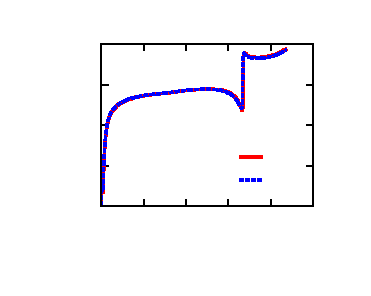
\includegraphics{ch-dynamics/conv_zst_U}}%
    \gplfronttext
  \end{picture}%
\endgroup

  \hspace{-0.40625in}
  % GNUPLOT: LaTeX picture with Postscript
\begingroup
  \makeatletter
  \providecommand\color[2][]{%
    \GenericError{(gnuplot) \space\space\space\@spaces}{%
      Package color not loaded in conjunction with
      terminal option `colourtext'%
    }{See the gnuplot documentation for explanation.%
    }{Either use 'blacktext' in gnuplot or load the package
      color.sty in LaTeX.}%
    \renewcommand\color[2][]{}%
  }%
  \providecommand\includegraphics[2][]{%
    \GenericError{(gnuplot) \space\space\space\@spaces}{%
      Package graphicx or graphics not loaded%
    }{See the gnuplot documentation for explanation.%
    }{The gnuplot epslatex terminal needs graphicx.sty or graphics.sty.}%
    \renewcommand\includegraphics[2][]{}%
  }%
  \providecommand\rotatebox[2]{#2}%
  \@ifundefined{ifGPcolor}{%
    \newif\ifGPcolor
    \GPcolortrue
  }{}%
  \@ifundefined{ifGPblacktext}{%
    \newif\ifGPblacktext
    \GPblacktexttrue
  }{}%
  % define a \g@addto@macro without @ in the name:
  \let\gplgaddtomacro\g@addto@macro
  % define empty templates for all commands taking text:
  \gdef\gplbacktext{}%
  \gdef\gplfronttext{}%
  \makeatother
  \ifGPblacktext
    % no textcolor at all
    \def\colorrgb#1{}%
    \def\colorgray#1{}%
  \else
    % gray or color?
    \ifGPcolor
      \def\colorrgb#1{\color[rgb]{#1}}%
      \def\colorgray#1{\color[gray]{#1}}%
      \expandafter\def\csname LTw\endcsname{\color{white}}%
      \expandafter\def\csname LTb\endcsname{\color{black}}%
      \expandafter\def\csname LTa\endcsname{\color{black}}%
      \expandafter\def\csname LT0\endcsname{\color[rgb]{1,0,0}}%
      \expandafter\def\csname LT1\endcsname{\color[rgb]{0,1,0}}%
      \expandafter\def\csname LT2\endcsname{\color[rgb]{0,0,1}}%
      \expandafter\def\csname LT3\endcsname{\color[rgb]{1,0,1}}%
      \expandafter\def\csname LT4\endcsname{\color[rgb]{0,1,1}}%
      \expandafter\def\csname LT5\endcsname{\color[rgb]{1,1,0}}%
      \expandafter\def\csname LT6\endcsname{\color[rgb]{0,0,0}}%
      \expandafter\def\csname LT7\endcsname{\color[rgb]{1,0.3,0}}%
      \expandafter\def\csname LT8\endcsname{\color[rgb]{0.5,0.5,0.5}}%
    \else
      % gray
      \def\colorrgb#1{\color{black}}%
      \def\colorgray#1{\color[gray]{#1}}%
      \expandafter\def\csname LTw\endcsname{\color{white}}%
      \expandafter\def\csname LTb\endcsname{\color{black}}%
      \expandafter\def\csname LTa\endcsname{\color{black}}%
      \expandafter\def\csname LT0\endcsname{\color{black}}%
      \expandafter\def\csname LT1\endcsname{\color{black}}%
      \expandafter\def\csname LT2\endcsname{\color{black}}%
      \expandafter\def\csname LT3\endcsname{\color{black}}%
      \expandafter\def\csname LT4\endcsname{\color{black}}%
      \expandafter\def\csname LT5\endcsname{\color{black}}%
      \expandafter\def\csname LT6\endcsname{\color{black}}%
      \expandafter\def\csname LT7\endcsname{\color{black}}%
      \expandafter\def\csname LT8\endcsname{\color{black}}%
    \fi
  \fi
  \setlength{\unitlength}{0.0500bp}%
  \begin{picture}(3600.00,2520.00)%
    \gplgaddtomacro\gplbacktext{%
      \csname LTb\endcsname%
      \put(1078,704){\makebox(0,0)[r]{\strut{} 600}}%
      \put(1078,1014){\makebox(0,0)[r]{\strut{} 1000}}%
      \put(1078,1325){\makebox(0,0)[r]{\strut{} 1400}}%
      \put(1078,1635){\makebox(0,0)[r]{\strut{} 1800}}%
      \put(1078,1946){\makebox(0,0)[r]{\strut{} 2200}}%
      \put(1078,2256){\makebox(0,0)[r]{\strut{} 2600}}%
      \put(1210,484){\makebox(0,0){\strut{} 0}}%
      \put(1609,484){\makebox(0,0){\strut{} 2}}%
      \put(2007,484){\makebox(0,0){\strut{} 4}}%
      \put(2406,484){\makebox(0,0){\strut{} 6}}%
      \put(2804,484){\makebox(0,0){\strut{} 8}}%
      \put(3203,484){\makebox(0,0){\strut{} 10}}%
      \put(176,1480){\rotatebox{-270}{\makebox(0,0){\strut{}\vspace{-48pt}$T$ [K]}}}%
      \put(2206,154){\makebox(0,0){\strut{}$x/D$}}%
      \put(1459,2023){\makebox(0,0)[l]{\strut{}Nominal}}%
      \put(1459,1790){\makebox(0,0)[l]{\strut{}Coarser}}%
    }%
    \gplgaddtomacro\gplfronttext{%
      \csname LTb\endcsname%
      \put(1871,2037){\makebox(0,0)[r]{\strut{} }}%
      \csname LTb\endcsname%
      \put(1871,1817){\makebox(0,0)[r]{\strut{} }}%
    }%
    \gplbacktext
    \put(0,0){
\includegraphics{conv_zst_T}}%
    \gplfronttext
  \end{picture}%
\endgroup

  \hspace{-0.40625in}
  % GNUPLOT: LaTeX picture with Postscript
\begingroup
  \makeatletter
  \providecommand\color[2][]{%
    \GenericError{(gnuplot) \space\space\space\@spaces}{%
      Package color not loaded in conjunction with
      terminal option `colourtext'%
    }{See the gnuplot documentation for explanation.%
    }{Either use 'blacktext' in gnuplot or load the package
      color.sty in LaTeX.}%
    \renewcommand\color[2][]{}%
  }%
  \providecommand\includegraphics[2][]{%
    \GenericError{(gnuplot) \space\space\space\@spaces}{%
      Package graphicx or graphics not loaded%
    }{See the gnuplot documentation for explanation.%
    }{The gnuplot epslatex terminal needs graphicx.sty or graphics.sty.}%
    \renewcommand\includegraphics[2][]{}%
  }%
  \providecommand\rotatebox[2]{#2}%
  \@ifundefined{ifGPcolor}{%
    \newif\ifGPcolor
    \GPcolortrue
  }{}%
  \@ifundefined{ifGPblacktext}{%
    \newif\ifGPblacktext
    \GPblacktexttrue
  }{}%
  % define a \g@addto@macro without @ in the name:
  \let\gplgaddtomacro\g@addto@macro
  % define empty templates for all commands taking text:
  \gdef\gplbacktext{}%
  \gdef\gplfronttext{}%
  \makeatother
  \ifGPblacktext
    % no textcolor at all
    \def\colorrgb#1{}%
    \def\colorgray#1{}%
  \else
    % gray or color?
    \ifGPcolor
      \def\colorrgb#1{\color[rgb]{#1}}%
      \def\colorgray#1{\color[gray]{#1}}%
      \expandafter\def\csname LTw\endcsname{\color{white}}%
      \expandafter\def\csname LTb\endcsname{\color{black}}%
      \expandafter\def\csname LTa\endcsname{\color{black}}%
      \expandafter\def\csname LT0\endcsname{\color[rgb]{1,0,0}}%
      \expandafter\def\csname LT1\endcsname{\color[rgb]{0,1,0}}%
      \expandafter\def\csname LT2\endcsname{\color[rgb]{0,0,1}}%
      \expandafter\def\csname LT3\endcsname{\color[rgb]{1,0,1}}%
      \expandafter\def\csname LT4\endcsname{\color[rgb]{0,1,1}}%
      \expandafter\def\csname LT5\endcsname{\color[rgb]{1,1,0}}%
      \expandafter\def\csname LT6\endcsname{\color[rgb]{0,0,0}}%
      \expandafter\def\csname LT7\endcsname{\color[rgb]{1,0.3,0}}%
      \expandafter\def\csname LT8\endcsname{\color[rgb]{0.5,0.5,0.5}}%
    \else
      % gray
      \def\colorrgb#1{\color{black}}%
      \def\colorgray#1{\color[gray]{#1}}%
      \expandafter\def\csname LTw\endcsname{\color{white}}%
      \expandafter\def\csname LTb\endcsname{\color{black}}%
      \expandafter\def\csname LTa\endcsname{\color{black}}%
      \expandafter\def\csname LT0\endcsname{\color{black}}%
      \expandafter\def\csname LT1\endcsname{\color{black}}%
      \expandafter\def\csname LT2\endcsname{\color{black}}%
      \expandafter\def\csname LT3\endcsname{\color{black}}%
      \expandafter\def\csname LT4\endcsname{\color{black}}%
      \expandafter\def\csname LT5\endcsname{\color{black}}%
      \expandafter\def\csname LT6\endcsname{\color{black}}%
      \expandafter\def\csname LT7\endcsname{\color{black}}%
      \expandafter\def\csname LT8\endcsname{\color{black}}%
    \fi
  \fi
  \setlength{\unitlength}{0.0500bp}%
  \begin{picture}(3744.00,2520.00)%
    \gplgaddtomacro\gplbacktext{%
      \csname LTb\endcsname%
      \put(1210,704){\makebox(0,0)[r]{\strut{} 0}}%
      \put(1210,1014){\makebox(0,0)[r]{\strut{} 0.002}}%
      \put(1210,1325){\makebox(0,0)[r]{\strut{} 0.004}}%
      \put(1210,1635){\makebox(0,0)[r]{\strut{} 0.006}}%
      \put(1210,1946){\makebox(0,0)[r]{\strut{} 0.008}}%
      \put(1210,2256){\makebox(0,0)[r]{\strut{} 0.01}}%
      \put(1342,484){\makebox(0,0){\strut{} 0}}%
      \put(1743,484){\makebox(0,0){\strut{} 2}}%
      \put(2144,484){\makebox(0,0){\strut{} 4}}%
      \put(2545,484){\makebox(0,0){\strut{} 6}}%
      \put(2946,484){\makebox(0,0){\strut{} 8}}%
      \put(3347,484){\makebox(0,0){\strut{} 10}}%
      \put(176,1480){\rotatebox{-270}{\makebox(0,0){\strut{}\vspace{-52pt}$Y_{\rm H_2O_2}$}}}%
      \put(2344,154){\makebox(0,0){\strut{}$x/D$}}%
      \put(1593,2023){\makebox(0,0)[l]{\strut{}Nominal}}%
      \put(1593,1790){\makebox(0,0)[l]{\strut{}Coarser}}%
    }%
    \gplgaddtomacro\gplfronttext{%
      \csname LTb\endcsname%
      \put(2035,2022){\makebox(0,0)[r]{\strut{} }}%
      \csname LTb\endcsname%
      \put(2035,1802){\makebox(0,0)[r]{\strut{} }}%
    }%
    \gplbacktext
    \put(0,0){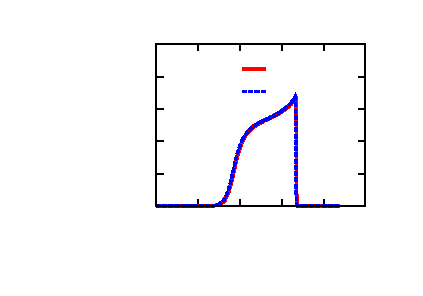
\includegraphics{conv_zst_H2O2}}%
    \gplfronttext
  \end{picture}%
\endgroup

%  \vspace{-0.1875in}
  \normalsize
  \caption{Velocity, temperature, and H$_2$O$_2$ profiles along $Z_{\rm st}$ on the nominal and two times coarser (in each direction) meshes for an air temperature of $800$ K.}
  \label{fig:convergence}
\end{figure}



\section{Thermal and Chemical Structure} 

\begin{figure}[t]
  \centering
  \scriptsize
  \vspace{-0.1in}
  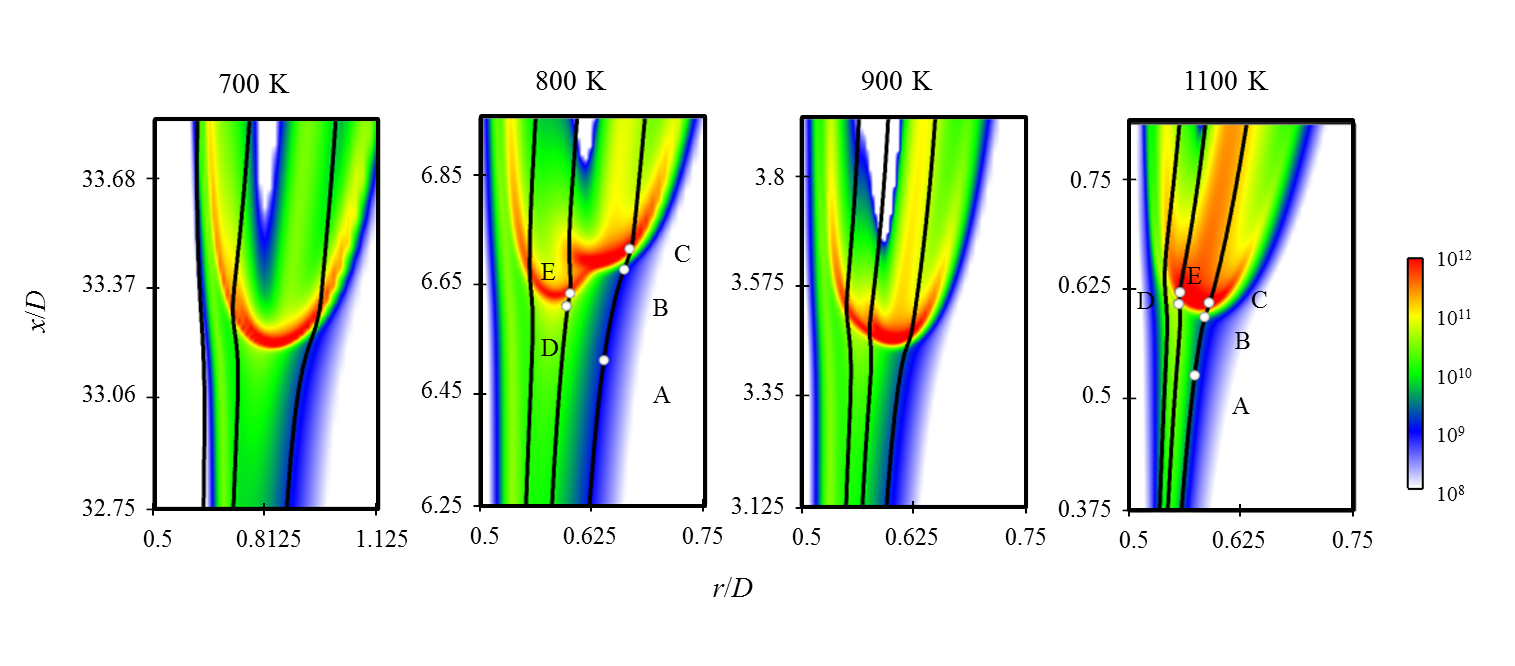
\includegraphics[width=1.0\textwidth]{HRR.png}
  \normalsize
  \vspace{-0.1in}
  \caption{Heat release rate [J/m$^3$-s] profiles.  The iso-contours of $Z_{\rm st}$, $Z = 0.2$, and $Z = 0.3$ are outlined from right to left in solid lines, respectively.  The CEMA sampling points at $800$ and $1100$ K are marked along the iso-contours.}
  \label{fig:HRR}
\end{figure}

To visualize the flame structures, the heat release rates profiles for the four cases ($700$, $800$, $900$, and $1100$ K) are shown in Fig.~\ref{fig:HRR}.  Qualitatively, the most upstream point on the largest heat release contour (the leading point), colored by red, will be referred to as the stabilization point.  

At $700$ K, a tribrachial thermal structure is observed, and the stabilization point locates around $Z = 0.15$, which is richer than the triple point, where the three branches intersect.  Moreover, compared to the classical triple flame structure, the middle heat release rate branch, corresponding to the nonpremixed flame, is significantly weaker than the other two branches.  

At $800$ K, the stabilization point is not located on the triple flame structure any more.  Instead, it is located near $Z = 0.23$ and connects two trailing heat release branches, where a tribrachial flame structure is attached to the leaner branch (LB) of the bibrachial reacting front.  A schematic of the structure is shown in Fig.~\ref{fig:schematic_800}.

\begin{figure}[t]
  \centering
  \scriptsize
%  \vspace{-0.1in}
  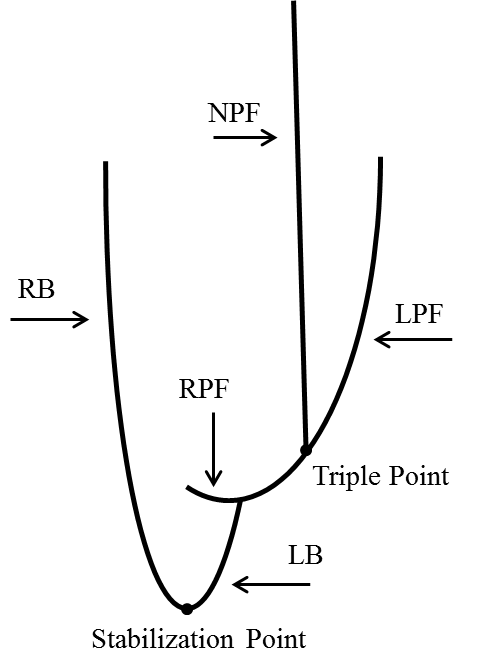
\includegraphics[width=0.4\textwidth]{schematic_800.png}
  \normalsize
%  \vspace{-0.1in}
  \caption{A schematic of the thermal structure of the $800$ K case.  LPF, RPF, and NPF denotes the lean premixed, rich premixed, and nonpremixed flame branch on the triple flame structure, respectively.  LB and RB denotes the leaner and richer branch of the reacting front, respectively.}
  \label{fig:schematic_800}
\end{figure}

As the air boundary temperature increases to $900$ K, the stabilization point shifts back to $Z = 0.14$.  Moreover, a long trailing branch at richer mixture fraction is attached to the main triple flame, resulting in a tetrabrachial structure.  Compared with the structure shown in the $800$ K case, the main triple flame stabilizes further upstream, as it depends less on the radical accumulation ahead of the flame.  Therefore, it catches up with the reacting front at richer mixture fraction, and they merge as the tetrabrachial structure.

A further increase in the boundary temperature results in a structure that is very similar to the classical triple flame, except for the fact that there is also heat release ahead of the stabilization point at $Z = 0.13$.  Some of the multibrachial structures were also observed by Krisman \emph{et al.}~\cite{krisman14}, using different definitions for branches, and it was concluded that the autoignition chemistry could affect the flame structure and the stabilization mechanism.  

To first qualitatively demonstrate the chemical structure of the flame, selected species profiles were examined, shown in~\Cref{fig:OH,fig:RO2,fig:HO2,fig:H2O2}.  The methoxymethylperoxy radical (CH$_3$OCH$_2$O$_2$) and hydroxyl radical (OH) were chosen as indicators of low and high temperature chemistry, respectively.  The hydroperoxyl radical (HO$_2$) and hydrogen peroxide (H$_2$O$_2$) were chosen, for they form in the preheat zone of a flame or before autoignition but quickly vanish in the post flame zone or after ignition~\cite{yoo09}.

For all four cases, similar profiles can be seen for some species.  First, the low temperature chemistry, which is indicated by the CH$_3$OCH$_2$O$_2$ radical, is found to be important at richer mixture fractions, where the temperature is lower.  Second, the OH radical peaks in the flame region and correlates well with the triple flame structure shown in the heat release rate profiles.  Third, HO$_2$ mass fraction peaks in a thin region.  Compared with the heat release rate contours, this thin region outlines the flame front and the reactive mixture at the rich mixture fractions and indicates the importance of the exothermic three-body recombination reaction H + O$_2$ + M $\Longleftrightarrow$ HO$_2$ + M.

However, there are also differences in the chemical structure among the different cases.  For example, for the $800$ and $900$ K cases, another OH local maxima, which is two orders of magnitudes smaller than the peak value on the triple flame, appears at richer mixture fractions, immediately downstream of where the CH$_3$OCH$_2$O$_2$ radical and H$_2$O$_2$ disappear, indicating autoignition.  Moreover, more pronounced differences between the three lower boundary temperature cases and the $1100$ K case are shown in the H$_2$O$_2$ profiles: for the lower boundary temperature cases, H$_2$O$_2$ accumulates along the mixture fraction iso-contours  until it decomposes in the flame region, while for the $1100$ K case, the H$_2$O$_2$ accumulation is an order of magnitude lower, due to the reduced residence time from the nozzle exit to the flame base.
  

\begin{figure}[t]
  \centering
  \scriptsize
  \vspace{-0.1in}
  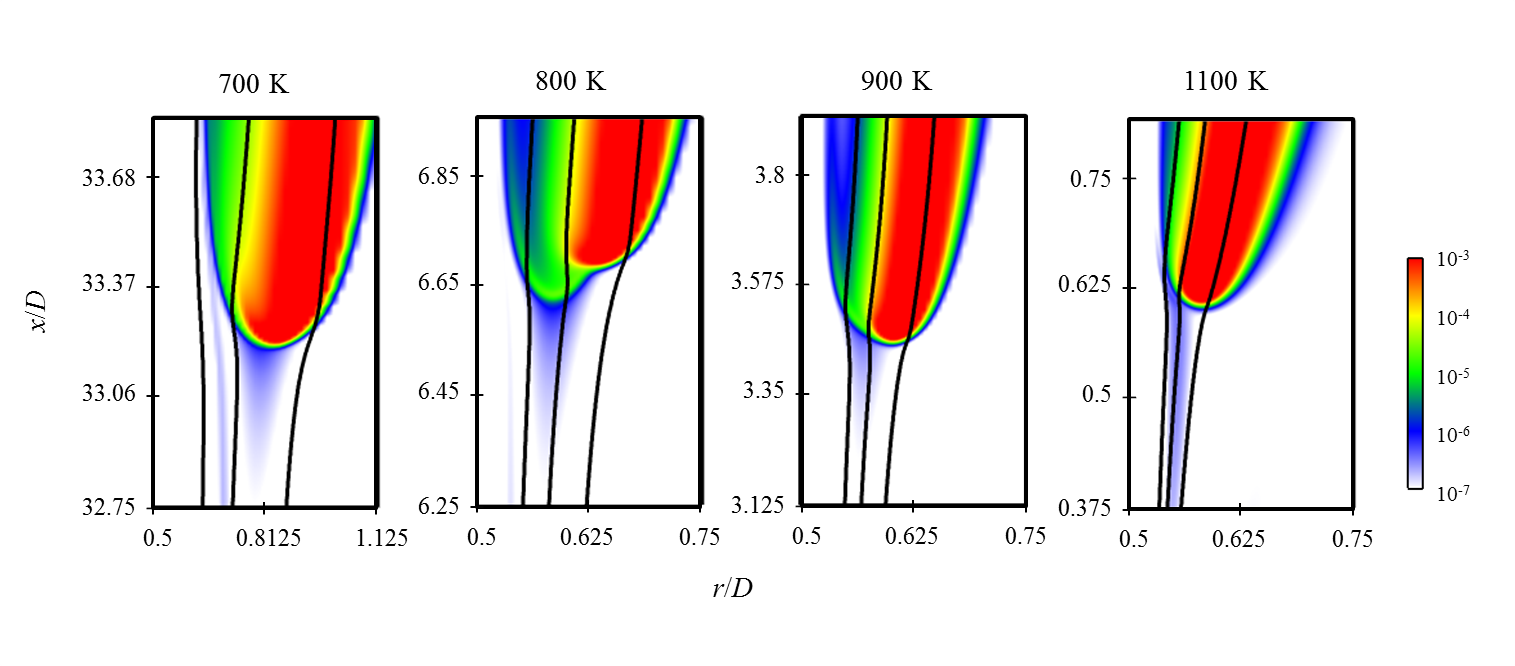
\includegraphics[width=1.0\textwidth]{OH.png}
  \normalsize
  \vspace{-0.1in}
  \caption{Hydroxyl radical mass fraction profiles.  The mixture fraction iso-contours are the same as in Fig.~\ref{fig:HRR}.}
  \label{fig:OH}
\end{figure}

\begin{figure}[t]
  \centering
  \scriptsize
  \vspace{-0.1in}
  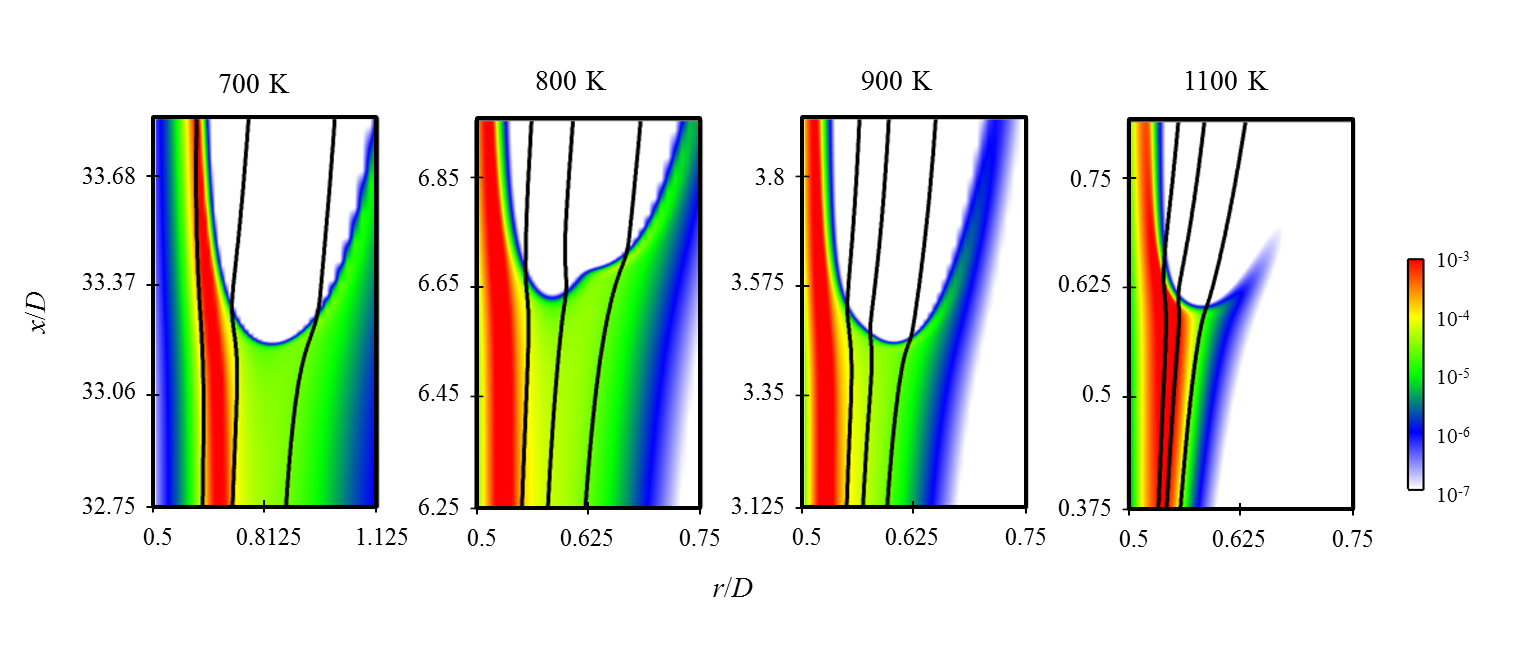
\includegraphics[width=1.0\textwidth]{RO2.png}
  \normalsize
  \vspace{-0.1in}
  \caption{Methoxymethylperoxy radical mass fraction profiles.  The mixture fraction iso-contours are the same as in Fig.~\ref{fig:HRR}.}
  \label{fig:RO2}
\end{figure}

\begin{figure}[t]
  \centering
  \scriptsize
  \vspace{-0.1in}
  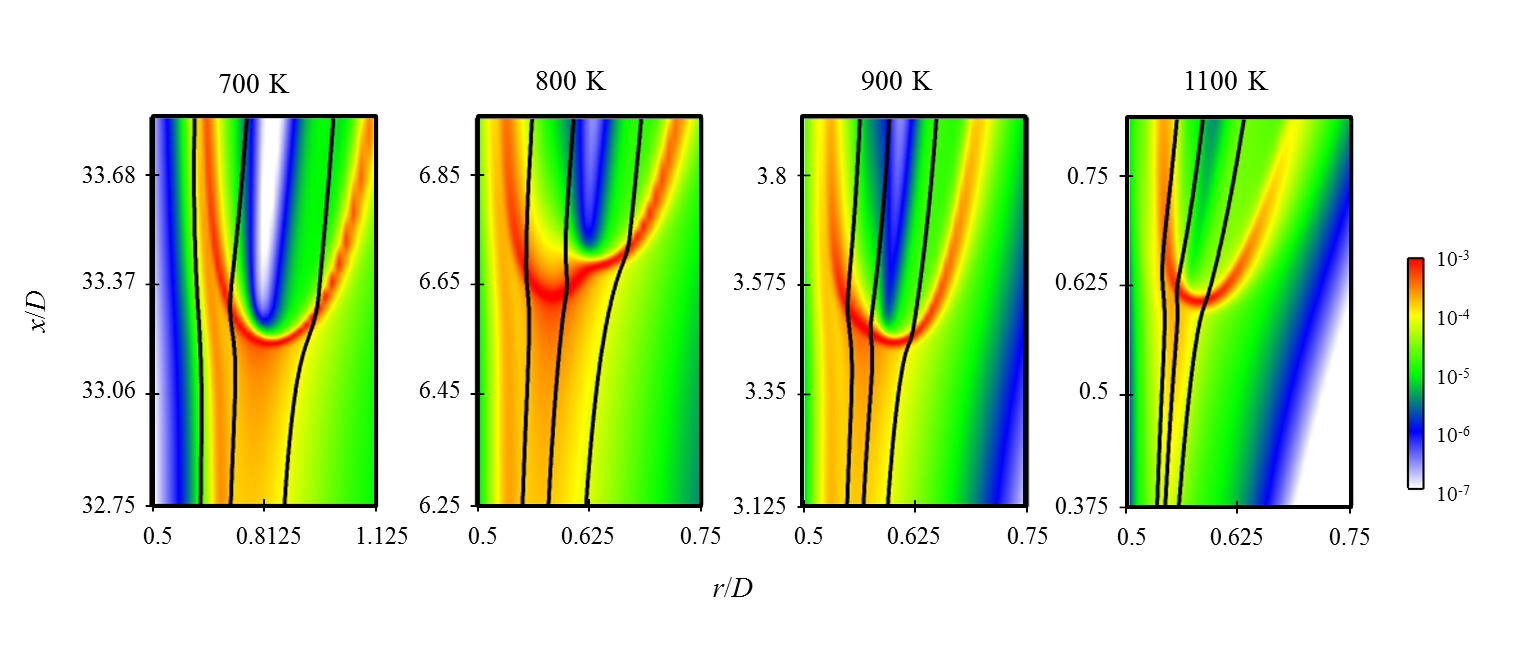
\includegraphics[width=1.0\textwidth]{HO2.png}
  \normalsize
  \vspace{-0.1in}
  \caption{Hydroperoxyl radical mass fraction profiles.  The mixture fraction iso-contours are the same as in Fig.~\ref{fig:HRR}.}
  \label{fig:HO2}
\end{figure}

\begin{figure}[t]
  \centering
  \scriptsize
  \vspace{-0.1in}
  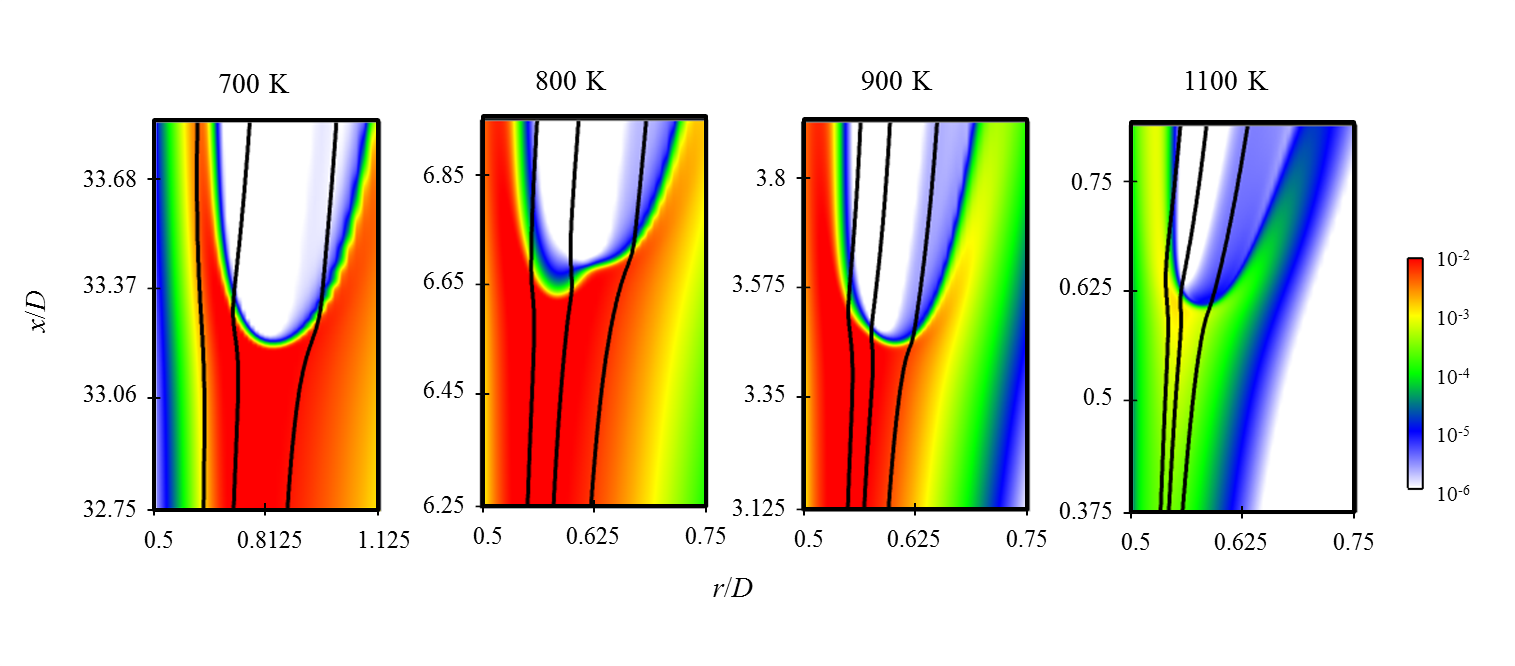
\includegraphics[width=1.0\textwidth]{H2O2.png}
  \normalsize
  \vspace{-0.1in}
  \caption{Hydrogen peroxide mass fraction profiles.  The mixture fraction iso-contours are the same as in Fig.~\ref{fig:HRR}.}
  \label{fig:H2O2}
\end{figure}

\section{Computational Diagnostics and Analysis}
The above heat release rate and speices profiles demonstrate the thermal and chemical structure of the reacting fronts at different boundary temperatures.  However, more detailed computational diagnostics and analysis are needed to further demonstrate the controlling chemistry and the stabilization mechanism.
\subsection{Chemical Explosive Mode Analysis}
In addition to the analysis based on selected species profiles, Chemical Explosive Mode Analysis (CEMA)~\cite{lu10,shan12} was conducted to identify the controlling chemistry in these complex reacting flows.  Briefly, the eigenvalues of the Jacobian matrix of the chemical source term based on the local species concentrations and temperature are evaluated and determined as the chemical modes.  The largest positive eigenvalue, which is defined as the chemical explosive mode, describes the rate of system runaway.  The projection of a reaction on the explosive mode is defined as the explosion participation index to account for its contribution to the explosive mode.  

In the present study, the dominant reactions at representative locations, such as those upstream and near the flame base are identified, based on the explosive mode and participation index.  For each case, the local species concentrations and temperature were sampled along the $Z_{\rm st}$, $Z = 0.2$, and $Z = 0.3$ iso-contours, as marked in Fig.~\ref{fig:HRR}, and processed by CEMA to demonstrate the evolution of the dominant reactions.

\begin{figure}
  \centering
  \scriptsize
  % GNUPLOT: LaTeX picture with Postscript
\begingroup
  \makeatletter
  \providecommand\color[2][]{%
    \GenericError{(gnuplot) \space\space\space\@spaces}{%
      Package color not loaded in conjunction with
      terminal option `colourtext'%
    }{See the gnuplot documentation for explanation.%
    }{Either use 'blacktext' in gnuplot or load the package
      color.sty in LaTeX.}%
    \renewcommand\color[2][]{}%
  }%
  \providecommand\includegraphics[2][]{%
    \GenericError{(gnuplot) \space\space\space\@spaces}{%
      Package graphicx or graphics not loaded%
    }{See the gnuplot documentation for explanation.%
    }{The gnuplot epslatex terminal needs graphicx.sty or graphics.sty.}%
    \renewcommand\includegraphics[2][]{}%
  }%
  \providecommand\rotatebox[2]{#2}%
  \@ifundefined{ifGPcolor}{%
    \newif\ifGPcolor
    \GPcolortrue
  }{}%
  \@ifundefined{ifGPblacktext}{%
    \newif\ifGPblacktext
    \GPblacktexttrue
  }{}%
  % define a \g@addto@macro without @ in the name:
  \let\gplgaddtomacro\g@addto@macro
  % define empty templates for all commands taking text:
  \gdef\gplbacktext{}%
  \gdef\gplfronttext{}%
  \makeatother
  \ifGPblacktext
    % no textcolor at all
    \def\colorrgb#1{}%
    \def\colorgray#1{}%
  \else
    % gray or color?
    \ifGPcolor
      \def\colorrgb#1{\color[rgb]{#1}}%
      \def\colorgray#1{\color[gray]{#1}}%
      \expandafter\def\csname LTw\endcsname{\color{white}}%
      \expandafter\def\csname LTb\endcsname{\color{black}}%
      \expandafter\def\csname LTa\endcsname{\color{black}}%
      \expandafter\def\csname LT0\endcsname{\color[rgb]{1,0,0}}%
      \expandafter\def\csname LT1\endcsname{\color[rgb]{0,1,0}}%
      \expandafter\def\csname LT2\endcsname{\color[rgb]{0,0,1}}%
      \expandafter\def\csname LT3\endcsname{\color[rgb]{1,0,1}}%
      \expandafter\def\csname LT4\endcsname{\color[rgb]{0,1,1}}%
      \expandafter\def\csname LT5\endcsname{\color[rgb]{1,1,0}}%
      \expandafter\def\csname LT6\endcsname{\color[rgb]{0,0,0}}%
      \expandafter\def\csname LT7\endcsname{\color[rgb]{1,0.3,0}}%
      \expandafter\def\csname LT8\endcsname{\color[rgb]{0.5,0.5,0.5}}%
    \else
      % gray
      \def\colorrgb#1{\color{black}}%
      \def\colorgray#1{\color[gray]{#1}}%
      \expandafter\def\csname LTw\endcsname{\color{white}}%
      \expandafter\def\csname LTb\endcsname{\color{black}}%
      \expandafter\def\csname LTa\endcsname{\color{black}}%
      \expandafter\def\csname LT0\endcsname{\color{black}}%
      \expandafter\def\csname LT1\endcsname{\color{black}}%
      \expandafter\def\csname LT2\endcsname{\color{black}}%
      \expandafter\def\csname LT3\endcsname{\color{black}}%
      \expandafter\def\csname LT4\endcsname{\color{black}}%
      \expandafter\def\csname LT5\endcsname{\color{black}}%
      \expandafter\def\csname LT6\endcsname{\color{black}}%
      \expandafter\def\csname LT7\endcsname{\color{black}}%
      \expandafter\def\csname LT8\endcsname{\color{black}}%
    \fi
  \fi
  \setlength{\unitlength}{0.0500bp}%
  \begin{picture}(7200.00,5040.00)%
    \gplgaddtomacro\gplbacktext{%
      \csname LTb\endcsname%
      \put(2748,1043){\makebox(0,0)[r]{\strut{}H$_2$O$_2$+M$\Longleftrightarrow$OH+OH+M}}%
      \put(2748,1383){\makebox(0,0)[r]{\strut{}HCO+O$_2$$\Longleftrightarrow$CO+HO$_2$}}%
      \put(2748,1722){\makebox(0,0)[r]{\strut{}CH$_2$OCH$_2$O$_2$H$\Longleftrightarrow$OH+CH$_2$O+CH$_2$O}}%
      \put(2748,2061){\makebox(0,0)[r]{\strut{}CH$_2$O+OH$\Longleftrightarrow$HCO+H$_2$O}}%
      \put(2748,2400){\makebox(0,0)[r]{\strut{}CH$_3$OCH$_3$+HO$_2$$\Longleftrightarrow$CH$_3$OCH$_2$+H$_2$O$_2$}}%
      \put(2748,2740){\makebox(0,0)[r]{\strut{}CH$_3$OCH$_2$+O$_2$$\Longleftrightarrow$CH$_3$OCH$_2$O$_2$}}%
      \put(2748,3079){\makebox(0,0)[r]{\strut{}HO$_2$+HO$_2$$\Longleftrightarrow$H$_2$O$_2$+O$_2$}}%
      \put(2748,3418){\makebox(0,0)[r]{\strut{}CH$_3$OCH$_2$O$_2$$\Longleftrightarrow$CH$_2$OCH$_2$O$_2$H}}%
      \put(2748,3757){\makebox(0,0)[r]{\strut{}H+O$_2$+M$\Longleftrightarrow$HO$_2$+M}}%
      \put(2748,4097){\makebox(0,0)[r]{\strut{}CH$_2$O+HO$_2$$\Longleftrightarrow$HCO+H$_2$O$_2$}}%
      \put(2748,4436){\makebox(0,0)[r]{\strut{}H+O$_2$$\Longleftrightarrow$O+OH}}%
      \put(2880,484){\makebox(0,0){\strut{}-1}}%
      \put(3861,484){\makebox(0,0){\strut{}-0.5}}%
      \put(4842,484){\makebox(0,0){\strut{} 0}}%
      \put(5822,484){\makebox(0,0){\strut{} 0.5}}%
      \put(6803,484){\makebox(0,0){\strut{} 1}}%
      \csname LTb\endcsname%
      \put(4841,154){\makebox(0,0){\strut{}Normalized Participation Index}}%
      \put(5234,1332){\makebox(0,0)[l]{\strut{}Point A}}%
      \put(5234,1501){\makebox(0,0)[l]{\strut{}Point B}}%
      \put(5234,1688){\makebox(0,0)[l]{\strut{}Point C}}%
      \put(5234,1857){\makebox(0,0)[l]{\strut{}Point D}}%
      \put(5234,2027){\makebox(0,0)[l]{\strut{}Point E}}%
      \put(5234,2231){\makebox(0,0)[l]{\strut{}$800$ K}}%
    }%
    \gplgaddtomacro\gplfronttext{%
      \csname LTb\endcsname%
      \put(5690,1337){\makebox(0,0)[r]{\strut{} }}%
      \csname LTb\endcsname%
      \put(5690,1513){\makebox(0,0)[r]{\strut{} }}%
      \csname LTb\endcsname%
      \put(5690,1689){\makebox(0,0)[r]{\strut{} }}%
      \csname LTb\endcsname%
      \put(5690,1865){\makebox(0,0)[r]{\strut{} }}%
      \csname LTb\endcsname%
      \put(5690,2041){\makebox(0,0)[r]{\strut{} }}%
    }%
    \gplbacktext
    \put(0,0){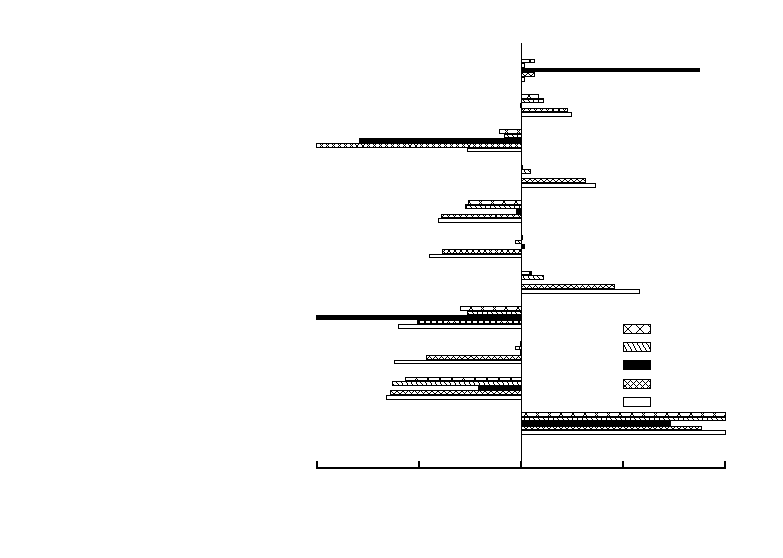
\includegraphics{CEMA_800}}%
    \gplfronttext
  \end{picture}%
\endgroup

  % GNUPLOT: LaTeX picture with Postscript
\begingroup
  \makeatletter
  \providecommand\color[2][]{%
    \GenericError{(gnuplot) \space\space\space\@spaces}{%
      Package color not loaded in conjunction with
      terminal option `colourtext'%
    }{See the gnuplot documentation for explanation.%
    }{Either use 'blacktext' in gnuplot or load the package
      color.sty in LaTeX.}%
    \renewcommand\color[2][]{}%
  }%
  \providecommand\includegraphics[2][]{%
    \GenericError{(gnuplot) \space\space\space\@spaces}{%
      Package graphicx or graphics not loaded%
    }{See the gnuplot documentation for explanation.%
    }{The gnuplot epslatex terminal needs graphicx.sty or graphics.sty.}%
    \renewcommand\includegraphics[2][]{}%
  }%
  \providecommand\rotatebox[2]{#2}%
  \@ifundefined{ifGPcolor}{%
    \newif\ifGPcolor
    \GPcolortrue
  }{}%
  \@ifundefined{ifGPblacktext}{%
    \newif\ifGPblacktext
    \GPblacktexttrue
  }{}%
  % define a \g@addto@macro without @ in the name:
  \let\gplgaddtomacro\g@addto@macro
  % define empty templates for all commands taking text:
  \gdef\gplbacktext{}%
  \gdef\gplfronttext{}%
  \makeatother
  \ifGPblacktext
    % no textcolor at all
    \def\colorrgb#1{}%
    \def\colorgray#1{}%
  \else
    % gray or color?
    \ifGPcolor
      \def\colorrgb#1{\color[rgb]{#1}}%
      \def\colorgray#1{\color[gray]{#1}}%
      \expandafter\def\csname LTw\endcsname{\color{white}}%
      \expandafter\def\csname LTb\endcsname{\color{black}}%
      \expandafter\def\csname LTa\endcsname{\color{black}}%
      \expandafter\def\csname LT0\endcsname{\color[rgb]{1,0,0}}%
      \expandafter\def\csname LT1\endcsname{\color[rgb]{0,1,0}}%
      \expandafter\def\csname LT2\endcsname{\color[rgb]{0,0,1}}%
      \expandafter\def\csname LT3\endcsname{\color[rgb]{1,0,1}}%
      \expandafter\def\csname LT4\endcsname{\color[rgb]{0,1,1}}%
      \expandafter\def\csname LT5\endcsname{\color[rgb]{1,1,0}}%
      \expandafter\def\csname LT6\endcsname{\color[rgb]{0,0,0}}%
      \expandafter\def\csname LT7\endcsname{\color[rgb]{1,0.3,0}}%
      \expandafter\def\csname LT8\endcsname{\color[rgb]{0.5,0.5,0.5}}%
    \else
      % gray
      \def\colorrgb#1{\color{black}}%
      \def\colorgray#1{\color[gray]{#1}}%
      \expandafter\def\csname LTw\endcsname{\color{white}}%
      \expandafter\def\csname LTb\endcsname{\color{black}}%
      \expandafter\def\csname LTa\endcsname{\color{black}}%
      \expandafter\def\csname LT0\endcsname{\color{black}}%
      \expandafter\def\csname LT1\endcsname{\color{black}}%
      \expandafter\def\csname LT2\endcsname{\color{black}}%
      \expandafter\def\csname LT3\endcsname{\color{black}}%
      \expandafter\def\csname LT4\endcsname{\color{black}}%
      \expandafter\def\csname LT5\endcsname{\color{black}}%
      \expandafter\def\csname LT6\endcsname{\color{black}}%
      \expandafter\def\csname LT7\endcsname{\color{black}}%
      \expandafter\def\csname LT8\endcsname{\color{black}}%
    \fi
  \fi
  \setlength{\unitlength}{0.0500bp}%
  \begin{picture}(7200.00,5040.00)%
    \gplgaddtomacro\gplbacktext{%
      \csname LTb\endcsname%
      \put(2748,1043){\makebox(0,0)[r]{\strut{}CH$_3$OCH$_2$$\Longleftrightarrow$CH$_2$O+CH$_3$}}%
      \put(2748,1383){\makebox(0,0)[r]{\strut{}CH$_3$OCH$_2$O$_2$$\Longleftrightarrow$CH$_2$OCH$_2$O$_2$H}}%
      \put(2748,1722){\makebox(0,0)[r]{\strut{}CH$_3$OCH$_3$+CH$_3$$\Longleftrightarrow$CH$_3$OCH$_2$+CH$_4$}}%
      \put(2748,2061){\makebox(0,0)[r]{\strut{}CH$_3$OCH$_3$+HO$_2$$\Longleftrightarrow$CH$_3$OCH$_2$+H$_2$O$_2$}}%
      \put(2748,2400){\makebox(0,0)[r]{\strut{}CH$_3$+CH$_3$+M$\Longleftrightarrow$C$_2$H$_6$+M}}%
      \put(2748,2740){\makebox(0,0)[r]{\strut{}CH$_3$+HO$_2$$\Longleftrightarrow$CH$_3$O+OH}}%
      \put(2748,3079){\makebox(0,0)[r]{\strut{}CH$_3$+HO$_2$$\Longleftrightarrow$CH$_4$+O$_2$}}%
      \put(2748,3418){\makebox(0,0)[r]{\strut{}CH$_2$OCH$_2$O$_2$H$\Longleftrightarrow$OH+CH$_2$O+CH$_2$O}}%
      \put(2748,3757){\makebox(0,0)[r]{\strut{}H$_2$O$_2$+M$\Longleftrightarrow$OH+OH+M}}%
      \put(2748,4097){\makebox(0,0)[r]{\strut{}H+O$_2$+M$\Longleftrightarrow$HO$_2$+M}}%
      \put(2748,4436){\makebox(0,0)[r]{\strut{}H+O$_2$$\Longleftrightarrow$O+OH}}%
      \put(2880,484){\makebox(0,0){\strut{}-1}}%
      \put(3861,484){\makebox(0,0){\strut{}-0.5}}%
      \put(4842,484){\makebox(0,0){\strut{} 0}}%
      \put(5822,484){\makebox(0,0){\strut{} 0.5}}%
      \put(6803,484){\makebox(0,0){\strut{} 1}}%
      \csname LTb\endcsname%
      \put(4841,154){\makebox(0,0){\strut{}Normalized Participation Index}}%
      \put(3076,1349){\makebox(0,0)[l]{\strut{}Point A}}%
      \put(3076,1518){\makebox(0,0)[l]{\strut{}Point B}}%
      \put(3076,1688){\makebox(0,0)[l]{\strut{}Point C}}%
      \put(3076,1857){\makebox(0,0)[l]{\strut{}Point D}}%
      \put(3076,2027){\makebox(0,0)[l]{\strut{}Point E}}%
      \put(3076,2231){\makebox(0,0)[l]{\strut{}$1100$ K}}%
    }%
    \gplgaddtomacro\gplfronttext{%
      \csname LTb\endcsname%
      \put(3532,1337){\makebox(0,0)[r]{\strut{} }}%
      \csname LTb\endcsname%
      \put(3532,1513){\makebox(0,0)[r]{\strut{} }}%
      \csname LTb\endcsname%
      \put(3532,1689){\makebox(0,0)[r]{\strut{} }}%
      \csname LTb\endcsname%
      \put(3532,1865){\makebox(0,0)[r]{\strut{} }}%
      \csname LTb\endcsname%
      \put(3532,2041){\makebox(0,0)[r]{\strut{} }}%
    }%
    \gplbacktext
    \put(0,0){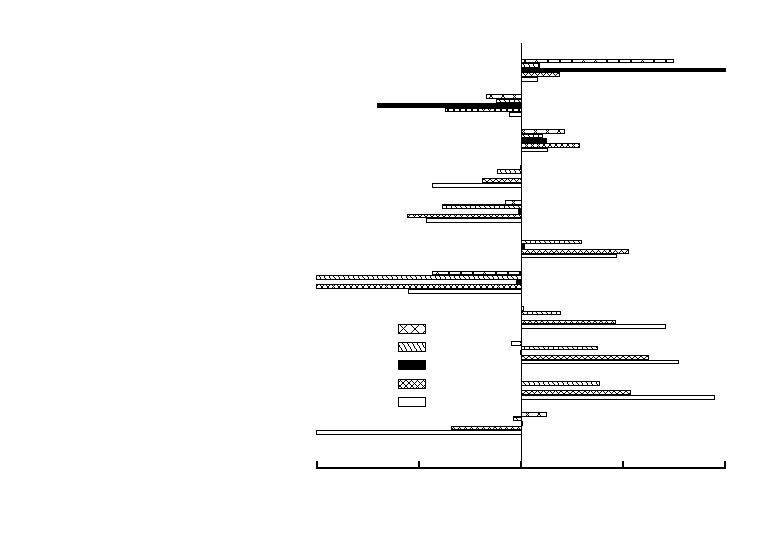
\includegraphics{CEMA_1100}}%
    \gplfronttext
  \end{picture}%
\endgroup

  \normalsize
  \caption{Normalized participation index at $800$ K and $1100$ K.  Sampled locations are marked in Fig.~\ref{fig:HRR}.}
  \label{fig:CEMA}
\end{figure}


The results are summarized in Fig.~\ref{fig:CEMA}, where three representative locations along the $Z_{\rm st}$ iso-contour approaching the flame front and two locations ahead of and at the reaction front at $Z = 0.2$ were sampled.  For the three lower coflow temperature cases, similar chemical patterns were found.  Upstream of the flame front, the eigenvalues of the chemical modes are positive, indicating that the mixtures have the potential to explode; after the flame front, the eigenvalues become negative, meaning that the mixtures are composed of burned products.  Following the $Z_{\rm st}$ iso-contour, the hydrogen peroxide chain branching reaction (H$_2$O$_2$ + M $\Longleftrightarrow$ OH + OH + M) is the reaction that has the largest projection on the explosive mode, showing the dominant role of autoignition chain branching.  The characteristic DME low temperature chemistry is also important upstream of the flame, where methoxymethylperoxy radical formation (CH$_3$OCH$_2$ + O$_2$ $\Longleftrightarrow$ CH$_3$OCH$_2$O$_2$) and isomerization (CH$_3$OCH$_2$O$_2$ $\Longleftrightarrow$ CH$_2$OCH$_2$O$_2$H) promote the explosion, while the $\beta$-scission reaction (CH$_2$OCH$_2$O$_2$H $\Longleftrightarrow$ OH + CH$_2$O + CH$_2$O) retards the explosion.  Approaching the flame front, the H radical recombination reaction (H + O$_2$ + M $\Longleftrightarrow$ HO$_2$ + M) becomes important for the $700-900$ K cases, due to the fact that the H radicals generated at the reaction zone diffuse upstream and undergo three-body recombination reactions under the high pressure, low temperature condition.  Further downstream where the heat release rate peaks, the hydrogen branching reaction (H + O$_2$ $\Longleftrightarrow$ O + OH) becomes the most important chain branching reaction, indicating that the combustion mode shifts from autoignition to flame propagation.  The nature of the tribrachial structure (around $Z_{\rm st}$) at $700-900$ K is therefore identified: an autoignition assisted premixed flame front.

CEMA conducted along the $Z = 0.2$ iso-contour, which crosses the rich heat release front in the $800$ and $900$ K cases, shows different chemical mode evolution.  The H$_2$O$_2$ chain branching reaction is always the dominant reaction that promotes the explosive mode, while the H radical recombination reaction and the H branching reaction is less important ahead of the rich heat release front and at the front.  Therefore, this heat release front is dominated by autoignition chemistry rather than flame chemistry and is considered as an autoignition front. 

On the contrary, although low temperature chemistry is still important for the $1100$ K case upstream of the reaction zone and the hydrogen chain branching reaction promotes explosion at the reaction zone, the hydrogen peroxide chain branching reaction is not very important for all the sampled locations.  Since the hydrogen peroxide reaction is the crucial chain branching reaction for the autoignition process, it is concluded that the $1100$ K case is less affected by autoignition chemistry than the lower boundary temperature cases.  

\subsection{Lagrangian Flamelet Analysis} \label{sec:LFA}
The above species profile analysis and CEMA results have demonstrated that autoignition chemistry is crucial to the complex flame structure in the $700$ to $900$ K cases.  However, the role that autoignition plays in the stabilization still needs further investigation.  To elucidate the role of autoignition for the current flow configuration, a direct comparison with the homogeneous counterpart for a Lagrangian flow particle is insufficient, for transport effects both parallel and perpendicular to the mixture fraction gradient are neglected.  First, the temperature and species stratification parallel to the mixture fraction gradient can significantly modify the ignition characteristics, especially for fuels with NTC chemistry~\cite{law12,deng14}.  Second, flame propagation perpendicular to the mixture fraction gradient can also influence the autoignition front through thermal and radical back diffusion. 

Unsteady flamelet analysis was conducted to account for diffusion parallel to mixture fraction gradients, and comparisons with the two-dimensional computations can then demonstrate the dominant stabilization mechanism.  If the thermal structure is stabilized by inhomogeneous autoignition, following the mixture fraction iso-contour, the spatial information from the two-dimensional computation could be interpreted as the time history of the corresponding mixture and predicted by the evolution of the flamelet.  Conversely, if premixed flame propagation is the dominant stabilization mechanism, the flamelet solution would not agree well with the two-dimensional computations, since the transport processes along the mixture fraction iso-contour are not negligible compared to the gradient direction. 

The unsteady flamelet model developed by Pitsch \emph{et al.}~\cite{pitsch98a}, referred to here as Lagrangian Flamelet Analysis (LFA), was adopted to investigate the evolution of the autoignitive mixing layer.  Due to mixing processes, the scalar dissipation rate $\chi$, which can influence the flamelet solution significantly, decreases in the streamwise direction.  Therefore, this dissipation rate variation must be considered when computing a flamelet as it evolves downstream.

In the present study, the unsteady flamelet was computed with FlameMaster~\cite{flamemaster}, and the dissipation rate was specified as a function of the flamelet time.  The flamelet time was computed from the NGA computational results, along the stoichiometric mixture fraction $Z_{\rm st}$ iso-contour: 
 \begin{equation} \label{eq:t}
t = \int ^{x}_{0} \frac{1}{(u + u_Z)(x')|(Z=Z_{\rm st})} dx'.
\end{equation}
This formulation is otherwise the same as that of Pitsch \emph {et al.}~\cite{pitsch98a}, except that, in addition to the axial component of the fluid convection velocity $u$, the axial component of the mixture fraction iso-contour propagation speed relative to the fluid convection $u_Z$ is also taken into account.  The expression for the constant property scalar iso-surface velocity relative to the local fluid motion was derived by Pope~\cite{pope88}, and the current work adopts the formulation derived by Lignell \emph {et al.}~\cite{lignell07} for variable properties:
\begin{equation}
\mathbf{u_Z} = -\frac{\nabla \cdot (\rho D_Z \nabla Z) }{\rho |\nabla Z|} \mathbf{n},
\end{equation}  
where $D_Z$ is the mixture fraction diffusivity and $\rho$ is the density.  The normal vector \textbf{n}, defined as
\begin{equation}
\mathbf{n} = \frac{\nabla Z}{|\nabla Z|},
\end{equation}
indicates the direction of this diffusion induced relative velocity.
The dissipation rate along the $Z_{\rm st} = 0.1005$ iso-contour obtained from the NGA computation was then correlated with this flamelet time and provided as the input for the FlameMaster calculation.  The dissipation rates at other mixture fractions were computed assuming the following form~\cite{petersbook}:
\begin{equation} \label{eq:Zref}
\chi{(Z)} = \chi{(Z_{\rm st})} \frac{\exp{(-2[{\rm erfc}^{-1}(2Z)]^2)}}{\exp{(-2[{\rm erfc}^{-1}(2Z_{\rm st})]^2)}} = \chi{(Z_{\rm st})} f(Z;Z_{\rm st}).
\end{equation}
To validate this formulation in the current configuration, the dissipation rates along different mixture fraction iso-contours were sampled from the NGA computations, normalized using Eq.~\ref{eq:Zref}, and compared with the sampling along the $Z_{\rm st}$ iso-contour.  As shown in Fig.~\ref{fig:Zref}, the normalized dissipation rates at different mixture fractions all collapse to the value at $Z_{\rm st}$.  Therefore, only the dissipation rate samplings along the $Z_{\rm st}$ iso-contour were needed to perform the unsteady flamelet calculation.

To account for the differential diffusion, species Lewis numbers for LFA  were specified the same as in the NGA computations.  The governing equations for species and temperature follow Eq. $24$ and $25$ in Pitsch and Peters~\cite{pitsch98b}.

\begin{figure}
  \centering
  \scriptsize
  % GNUPLOT: LaTeX picture with Postscript
\begingroup
  \makeatletter
  \providecommand\color[2][]{%
    \GenericError{(gnuplot) \space\space\space\@spaces}{%
      Package color not loaded in conjunction with
      terminal option `colourtext'%
    }{See the gnuplot documentation for explanation.%
    }{Either use 'blacktext' in gnuplot or load the package
      color.sty in LaTeX.}%
    \renewcommand\color[2][]{}%
  }%
  \providecommand\includegraphics[2][]{%
    \GenericError{(gnuplot) \space\space\space\@spaces}{%
      Package graphicx or graphics not loaded%
    }{See the gnuplot documentation for explanation.%
    }{The gnuplot epslatex terminal needs graphicx.sty or graphics.sty.}%
    \renewcommand\includegraphics[2][]{}%
  }%
  \providecommand\rotatebox[2]{#2}%
  \@ifundefined{ifGPcolor}{%
    \newif\ifGPcolor
    \GPcolortrue
  }{}%
  \@ifundefined{ifGPblacktext}{%
    \newif\ifGPblacktext
    \GPblacktexttrue
  }{}%
  % define a \g@addto@macro without @ in the name:
  \let\gplgaddtomacro\g@addto@macro
  % define empty templates for all commands taking text:
  \gdef\gplbacktext{}%
  \gdef\gplfronttext{}%
  \makeatother
  \ifGPblacktext
    % no textcolor at all
    \def\colorrgb#1{}%
    \def\colorgray#1{}%
  \else
    % gray or color?
    \ifGPcolor
      \def\colorrgb#1{\color[rgb]{#1}}%
      \def\colorgray#1{\color[gray]{#1}}%
      \expandafter\def\csname LTw\endcsname{\color{white}}%
      \expandafter\def\csname LTb\endcsname{\color{black}}%
      \expandafter\def\csname LTa\endcsname{\color{black}}%
      \expandafter\def\csname LT0\endcsname{\color[rgb]{1,0,0}}%
      \expandafter\def\csname LT1\endcsname{\color[rgb]{0,1,0}}%
      \expandafter\def\csname LT2\endcsname{\color[rgb]{0,0,1}}%
      \expandafter\def\csname LT3\endcsname{\color[rgb]{1,0,1}}%
      \expandafter\def\csname LT4\endcsname{\color[rgb]{0,1,1}}%
      \expandafter\def\csname LT5\endcsname{\color[rgb]{1,1,0}}%
      \expandafter\def\csname LT6\endcsname{\color[rgb]{0,0,0}}%
      \expandafter\def\csname LT7\endcsname{\color[rgb]{1,0.3,0}}%
      \expandafter\def\csname LT8\endcsname{\color[rgb]{0.5,0.5,0.5}}%
    \else
      % gray
      \def\colorrgb#1{\color{black}}%
      \def\colorgray#1{\color[gray]{#1}}%
      \expandafter\def\csname LTw\endcsname{\color{white}}%
      \expandafter\def\csname LTb\endcsname{\color{black}}%
      \expandafter\def\csname LTa\endcsname{\color{black}}%
      \expandafter\def\csname LT0\endcsname{\color{black}}%
      \expandafter\def\csname LT1\endcsname{\color{black}}%
      \expandafter\def\csname LT2\endcsname{\color{black}}%
      \expandafter\def\csname LT3\endcsname{\color{black}}%
      \expandafter\def\csname LT4\endcsname{\color{black}}%
      \expandafter\def\csname LT5\endcsname{\color{black}}%
      \expandafter\def\csname LT6\endcsname{\color{black}}%
      \expandafter\def\csname LT7\endcsname{\color{black}}%
      \expandafter\def\csname LT8\endcsname{\color{black}}%
    \fi
  \fi
  \setlength{\unitlength}{0.0500bp}%
  \begin{picture}(7200.00,5040.00)%
    \gplgaddtomacro\gplbacktext{%
      \csname LTb\endcsname%
      \put(946,704){\makebox(0,0)[r]{\strut{} 0}}%
      \put(946,1383){\makebox(0,0)[r]{\strut{} 50}}%
      \put(946,2061){\makebox(0,0)[r]{\strut{} 100}}%
      \put(946,2740){\makebox(0,0)[r]{\strut{} 150}}%
      \put(946,3418){\makebox(0,0)[r]{\strut{} 200}}%
      \put(946,4097){\makebox(0,0)[r]{\strut{} 250}}%
      \put(946,4775){\makebox(0,0)[r]{\strut{} 300}}%
      \put(1078,484){\makebox(0,0){\strut{} 0}}%
      \put(1841,484){\makebox(0,0){\strut{} 0.2}}%
      \put(2605,484){\makebox(0,0){\strut{} 0.4}}%
      \put(3368,484){\makebox(0,0){\strut{} 0.6}}%
      \put(4131,484){\makebox(0,0){\strut{} 0.8}}%
      \put(4895,484){\makebox(0,0){\strut{} 1}}%
      \put(5658,484){\makebox(0,0){\strut{} 1.2}}%
      \put(6421,484){\makebox(0,0){\strut{} 1.4}}%
      \put(176,2739){\rotatebox{-270}{\makebox(0,0){\strut{}\vspace{-28pt}$\frac{\chi(Z)}{f(Z,Z_{\rm st})}$ [1/s]}}}%
      \put(3940,154){\makebox(0,0){\strut{}Time [ms]}}%
    }%
    \gplgaddtomacro\gplfronttext{%
      \csname LTb\endcsname%
      \put(5816,4602){\makebox(0,0)[r]{\strut{}$Z = Z_{\rm st}$}}%
      \csname LTb\endcsname%
      \put(5816,4382){\makebox(0,0)[r]{\strut{}$Z = 0.2$}}%
      \csname LTb\endcsname%
      \put(5816,4162){\makebox(0,0)[r]{\strut{}$Z = 0.4$}}%
      \csname LTb\endcsname%
      \put(5816,3942){\makebox(0,0)[r]{\strut{}$Z = 0.6$}}%
    }%
    \gplbacktext
    \put(0,0){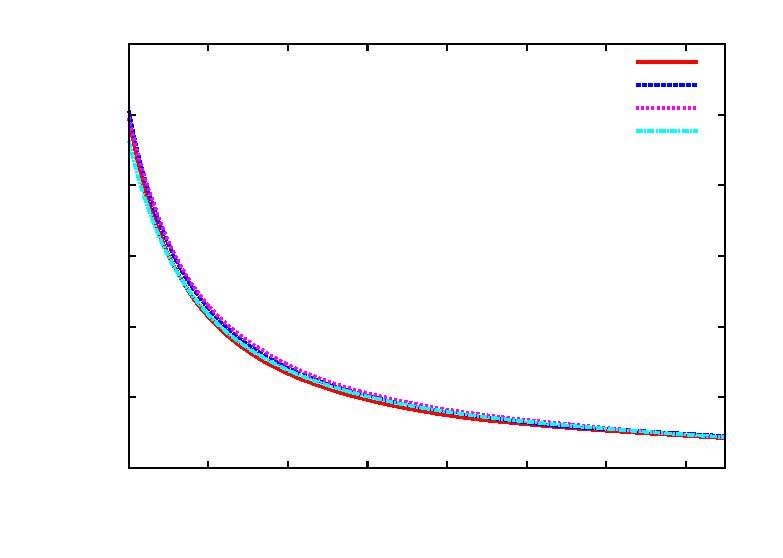
\includegraphics{Zref}}%
    \gplfronttext
  \end{picture}%
\endgroup

  \normalsize
  \caption{$\frac{\chi(Z)}{f(Z;Z_{\rm st})}$, using Eq.~\ref{eq:Zref}, based on NGA computation at $800$ K.}
  \label{fig:Zref}
\end{figure}

In the current work, the time history of the dissipation rate $\chi_{\rm st}$ was specified in FlameMaster according to the NGA computation.  To avoid the ill-defined Lagrangian time in the recirculation zone, time zero was defined at a downstream location ten times the thickness of the wall.  Accordingly, the species and temperature profiles along the radial cut at this location were specified as the initial conditions for the flamelet.  Based on these initial conditions and $\chi_{\rm st}$ time history profiles, the unsteady flamelets were calculated and compared with the two-dimensional computational results for $Z_{\rm st}$, $Z = 0.2$, and $Z = 0.3$.       

\begin{figure}
  \centering
  \scriptsize
  % GNUPLOT: LaTeX picture with Postscript
\begingroup
  \makeatletter
  \providecommand\color[2][]{%
    \GenericError{(gnuplot) \space\space\space\@spaces}{%
      Package color not loaded in conjunction with
      terminal option `colourtext'%
    }{See the gnuplot documentation for explanation.%
    }{Either use 'blacktext' in gnuplot or load the package
      color.sty in LaTeX.}%
    \renewcommand\color[2][]{}%
  }%
  \providecommand\includegraphics[2][]{%
    \GenericError{(gnuplot) \space\space\space\@spaces}{%
      Package graphicx or graphics not loaded%
    }{See the gnuplot documentation for explanation.%
    }{The gnuplot epslatex terminal needs graphicx.sty or graphics.sty.}%
    \renewcommand\includegraphics[2][]{}%
  }%
  \providecommand\rotatebox[2]{#2}%
  \@ifundefined{ifGPcolor}{%
    \newif\ifGPcolor
    \GPcolortrue
  }{}%
  \@ifundefined{ifGPblacktext}{%
    \newif\ifGPblacktext
    \GPblacktexttrue
  }{}%
  % define a \g@addto@macro without @ in the name:
  \let\gplgaddtomacro\g@addto@macro
  % define empty templates for all commands taking text:
  \gdef\gplbacktext{}%
  \gdef\gplfronttext{}%
  \makeatother
  \ifGPblacktext
    % no textcolor at all
    \def\colorrgb#1{}%
    \def\colorgray#1{}%
  \else
    % gray or color?
    \ifGPcolor
      \def\colorrgb#1{\color[rgb]{#1}}%
      \def\colorgray#1{\color[gray]{#1}}%
      \expandafter\def\csname LTw\endcsname{\color{white}}%
      \expandafter\def\csname LTb\endcsname{\color{black}}%
      \expandafter\def\csname LTa\endcsname{\color{black}}%
      \expandafter\def\csname LT0\endcsname{\color[rgb]{1,0,0}}%
      \expandafter\def\csname LT1\endcsname{\color[rgb]{0,1,0}}%
      \expandafter\def\csname LT2\endcsname{\color[rgb]{0,0,1}}%
      \expandafter\def\csname LT3\endcsname{\color[rgb]{1,0,1}}%
      \expandafter\def\csname LT4\endcsname{\color[rgb]{0,1,1}}%
      \expandafter\def\csname LT5\endcsname{\color[rgb]{1,1,0}}%
      \expandafter\def\csname LT6\endcsname{\color[rgb]{0,0,0}}%
      \expandafter\def\csname LT7\endcsname{\color[rgb]{1,0.3,0}}%
      \expandafter\def\csname LT8\endcsname{\color[rgb]{0.5,0.5,0.5}}%
    \else
      % gray
      \def\colorrgb#1{\color{black}}%
      \def\colorgray#1{\color[gray]{#1}}%
      \expandafter\def\csname LTw\endcsname{\color{white}}%
      \expandafter\def\csname LTb\endcsname{\color{black}}%
      \expandafter\def\csname LTa\endcsname{\color{black}}%
      \expandafter\def\csname LT0\endcsname{\color{black}}%
      \expandafter\def\csname LT1\endcsname{\color{black}}%
      \expandafter\def\csname LT2\endcsname{\color{black}}%
      \expandafter\def\csname LT3\endcsname{\color{black}}%
      \expandafter\def\csname LT4\endcsname{\color{black}}%
      \expandafter\def\csname LT5\endcsname{\color{black}}%
      \expandafter\def\csname LT6\endcsname{\color{black}}%
      \expandafter\def\csname LT7\endcsname{\color{black}}%
      \expandafter\def\csname LT8\endcsname{\color{black}}%
    \fi
  \fi
  \setlength{\unitlength}{0.0500bp}%
  \begin{picture}(11520.00,6048.00)%
    \gplgaddtomacro\gplbacktext{%
      \csname LTb\endcsname%
      \put(7990,4756){\makebox(0,0)[r]{\strut{} 800}}%
      \put(7990,4961){\makebox(0,0)[r]{\strut{} 1200}}%
      \put(7990,5167){\makebox(0,0)[r]{\strut{} 1600}}%
      \put(7990,5372){\makebox(0,0)[r]{\strut{} 2000}}%
      \put(7990,5578){\makebox(0,0)[r]{\strut{} 2400}}%
      \put(7990,5783){\makebox(0,0)[r]{\strut{} 2800}}%
      \put(8122,4536){\makebox(0,0){\strut{} 0}}%
      \put(8440,4536){\makebox(0,0){\strut{} 0.25}}%
      \put(8759,4536){\makebox(0,0){\strut{} 0.5}}%
      \put(9077,4536){\makebox(0,0){\strut{} 0.75}}%
      \put(9395,4536){\makebox(0,0){\strut{} 1}}%
      \put(7088,5269){\rotatebox{-270}{\makebox(0,0){\strut{}\vspace{-48pt}$T$ [K]}}}%
      \put(8758,4206){\makebox(0,0){\strut{}\vspace{12pt}Time [ms]}}%
      \put(1728,6047){\makebox(0,0)[l]{\strut{}$700$ K}}%
      \put(4032,6047){\makebox(0,0)[l]{\strut{}$800$ K}}%
      \put(6335,6047){\makebox(0,0)[l]{\strut{}$900$ K}}%
      \put(8639,6047){\makebox(0,0)[l]{\strut{}$1100$ K}}%
      \put(-229,1209){\makebox(0,0)[l]{\strut{}$Z = 0.3$}}%
      \put(-229,3205){\makebox(0,0)[l]{\strut{}$Z = 0.2$}}%
      \put(-229,5261){\makebox(0,0)[l]{\strut{}$Z = Z_{\rm st}$}}%
    }%
    \gplgaddtomacro\gplfronttext{%
    }%
    \gplgaddtomacro\gplbacktext{%
      \csname LTb\endcsname%
      \put(7990,2941){\makebox(0,0)[r]{\strut{} 800}}%
      \put(7990,3147){\makebox(0,0)[r]{\strut{} 1200}}%
      \put(7990,3352){\makebox(0,0)[r]{\strut{} 1600}}%
      \put(7990,3558){\makebox(0,0)[r]{\strut{} 2000}}%
      \put(7990,3763){\makebox(0,0)[r]{\strut{} 2400}}%
      \put(7990,3969){\makebox(0,0)[r]{\strut{} 2800}}%
      \put(8122,2721){\makebox(0,0){\strut{} 0}}%
      \put(8440,2721){\makebox(0,0){\strut{} 0.25}}%
      \put(8759,2721){\makebox(0,0){\strut{} 0.5}}%
      \put(9077,2721){\makebox(0,0){\strut{} 0.75}}%
      \put(9395,2721){\makebox(0,0){\strut{} 1}}%
      \put(7088,3455){\rotatebox{-270}{\makebox(0,0){\strut{}\vspace{-48pt}$T$ [K]}}}%
      \put(8758,2391){\makebox(0,0){\strut{}\vspace{12pt}Time [ms]}}%
    }%
    \gplgaddtomacro\gplfronttext{%
    }%
    \gplgaddtomacro\gplbacktext{%
      \csname LTb\endcsname%
      \put(7990,1187){\makebox(0,0)[r]{\strut{} 400}}%
      \put(7990,1393){\makebox(0,0)[r]{\strut{} 800}}%
      \put(7990,1598){\makebox(0,0)[r]{\strut{} 1200}}%
      \put(7990,1804){\makebox(0,0)[r]{\strut{} 1600}}%
      \put(7990,2009){\makebox(0,0)[r]{\strut{} 2000}}%
      \put(7990,2215){\makebox(0,0)[r]{\strut{} 2400}}%
      \put(8122,967){\makebox(0,0){\strut{} 0}}%
      \put(8440,967){\makebox(0,0){\strut{} 0.25}}%
      \put(8759,967){\makebox(0,0){\strut{} 0.5}}%
      \put(9077,967){\makebox(0,0){\strut{} 0.75}}%
      \put(9395,967){\makebox(0,0){\strut{} 1}}%
      \put(7088,1701){\rotatebox{-270}{\makebox(0,0){\strut{}\vspace{-48pt}$T$ [K]}}}%
      \put(8758,637){\makebox(0,0){\strut{}\vspace{12pt}Time [ms]}}%
    }%
    \gplgaddtomacro\gplfronttext{%
    }%
    \gplgaddtomacro\gplbacktext{%
      \csname LTb\endcsname%
      \put(5686,4756){\makebox(0,0)[r]{\strut{} 600}}%
      \put(5686,4961){\makebox(0,0)[r]{\strut{} 1000}}%
      \put(5686,5167){\makebox(0,0)[r]{\strut{} 1400}}%
      \put(5686,5372){\makebox(0,0)[r]{\strut{} 1800}}%
      \put(5686,5578){\makebox(0,0)[r]{\strut{} 2200}}%
      \put(5686,5783){\makebox(0,0)[r]{\strut{} 2600}}%
      \put(5818,4536){\makebox(0,0){\strut{} 0}}%
      \put(6136,4536){\makebox(0,0){\strut{} 0.3}}%
      \put(6455,4536){\makebox(0,0){\strut{} 0.6}}%
      \put(6773,4536){\makebox(0,0){\strut{} 0.9}}%
      \put(7091,4536){\makebox(0,0){\strut{} 1.2}}%
      \put(4784,5269){\rotatebox{-270}{\makebox(0,0){\strut{}\vspace{-48pt}$T$ [K]}}}%
      \put(6454,4206){\makebox(0,0){\strut{}\vspace{12pt}Time [ms]}}%
    }%
    \gplgaddtomacro\gplfronttext{%
    }%
    \gplgaddtomacro\gplbacktext{%
      \csname LTb\endcsname%
      \put(5686,2941){\makebox(0,0)[r]{\strut{} 600}}%
      \put(5686,3147){\makebox(0,0)[r]{\strut{} 1000}}%
      \put(5686,3352){\makebox(0,0)[r]{\strut{} 1400}}%
      \put(5686,3558){\makebox(0,0)[r]{\strut{} 1800}}%
      \put(5686,3763){\makebox(0,0)[r]{\strut{} 2200}}%
      \put(5686,3969){\makebox(0,0)[r]{\strut{} 2600}}%
      \put(5818,2721){\makebox(0,0){\strut{} 0}}%
      \put(6136,2721){\makebox(0,0){\strut{} 0.3}}%
      \put(6455,2721){\makebox(0,0){\strut{} 0.6}}%
      \put(6773,2721){\makebox(0,0){\strut{} 0.9}}%
      \put(7091,2721){\makebox(0,0){\strut{} 1.2}}%
      \put(4784,3455){\rotatebox{-270}{\makebox(0,0){\strut{}\vspace{-48pt}$T$ [K]}}}%
      \put(6454,2391){\makebox(0,0){\strut{}\vspace{12pt}Time [ms]}}%
    }%
    \gplgaddtomacro\gplfronttext{%
    }%
    \gplgaddtomacro\gplbacktext{%
      \csname LTb\endcsname%
      \put(5686,1187){\makebox(0,0)[r]{\strut{} 400}}%
      \put(5686,1393){\makebox(0,0)[r]{\strut{} 800}}%
      \put(5686,1598){\makebox(0,0)[r]{\strut{} 1200}}%
      \put(5686,1804){\makebox(0,0)[r]{\strut{} 1600}}%
      \put(5686,2009){\makebox(0,0)[r]{\strut{} 2000}}%
      \put(5686,2215){\makebox(0,0)[r]{\strut{} 2400}}%
      \put(5818,967){\makebox(0,0){\strut{} 0}}%
      \put(6136,967){\makebox(0,0){\strut{} 0.3}}%
      \put(6455,967){\makebox(0,0){\strut{} 0.6}}%
      \put(6773,967){\makebox(0,0){\strut{} 0.9}}%
      \put(7091,967){\makebox(0,0){\strut{} 1.2}}%
      \put(4784,1701){\rotatebox{-270}{\makebox(0,0){\strut{}\vspace{-48pt}$T$ [K]}}}%
      \put(6454,637){\makebox(0,0){\strut{}\vspace{12pt}Time [ms]}}%
    }%
    \gplgaddtomacro\gplfronttext{%
    }%
    \gplgaddtomacro\gplbacktext{%
      \csname LTb\endcsname%
      \put(3382,4756){\makebox(0,0)[r]{\strut{} 600}}%
      \put(3382,4961){\makebox(0,0)[r]{\strut{} 1000}}%
      \put(3382,5167){\makebox(0,0)[r]{\strut{} 1400}}%
      \put(3382,5372){\makebox(0,0)[r]{\strut{} 1800}}%
      \put(3382,5578){\makebox(0,0)[r]{\strut{} 2200}}%
      \put(3382,5783){\makebox(0,0)[r]{\strut{} 2600}}%
      \put(3514,4536){\makebox(0,0){\strut{} 0}}%
      \put(3832,4536){\makebox(0,0){\strut{} 0.6}}%
      \put(4151,4536){\makebox(0,0){\strut{} 1.2}}%
      \put(4469,4536){\makebox(0,0){\strut{} 1.8}}%
      \put(4787,4536){\makebox(0,0){\strut{} 2.4}}%
      \put(2480,5269){\rotatebox{-270}{\makebox(0,0){\strut{}\vspace{-48pt}$T$ [K]}}}%
      \put(4150,4206){\makebox(0,0){\strut{}\vspace{12pt}Time [ms]}}%
    }%
    \gplgaddtomacro\gplfronttext{%
    }%
    \gplgaddtomacro\gplbacktext{%
      \csname LTb\endcsname%
      \put(3382,2941){\makebox(0,0)[r]{\strut{} 600}}%
      \put(3382,3147){\makebox(0,0)[r]{\strut{} 1000}}%
      \put(3382,3352){\makebox(0,0)[r]{\strut{} 1400}}%
      \put(3382,3558){\makebox(0,0)[r]{\strut{} 1800}}%
      \put(3382,3763){\makebox(0,0)[r]{\strut{} 2200}}%
      \put(3382,3969){\makebox(0,0)[r]{\strut{} 2600}}%
      \put(3514,2721){\makebox(0,0){\strut{} 0}}%
      \put(3832,2721){\makebox(0,0){\strut{} 0.6}}%
      \put(4151,2721){\makebox(0,0){\strut{} 1.2}}%
      \put(4469,2721){\makebox(0,0){\strut{} 1.8}}%
      \put(4787,2721){\makebox(0,0){\strut{} 2.4}}%
      \put(2480,3455){\rotatebox{-270}{\makebox(0,0){\strut{}\vspace{-48pt}$T$ [K]}}}%
      \put(4150,2391){\makebox(0,0){\strut{}\vspace{12pt}Time [ms]}}%
    }%
    \gplgaddtomacro\gplfronttext{%
    }%
    \gplgaddtomacro\gplbacktext{%
      \csname LTb\endcsname%
      \put(3382,1187){\makebox(0,0)[r]{\strut{} 400}}%
      \put(3382,1393){\makebox(0,0)[r]{\strut{} 800}}%
      \put(3382,1598){\makebox(0,0)[r]{\strut{} 1200}}%
      \put(3382,1804){\makebox(0,0)[r]{\strut{} 1600}}%
      \put(3382,2009){\makebox(0,0)[r]{\strut{} 2000}}%
      \put(3382,2215){\makebox(0,0)[r]{\strut{} 2400}}%
      \put(3514,967){\makebox(0,0){\strut{} 0}}%
      \put(3832,967){\makebox(0,0){\strut{} 0.6}}%
      \put(4151,967){\makebox(0,0){\strut{} 1.2}}%
      \put(4469,967){\makebox(0,0){\strut{} 1.8}}%
      \put(4787,967){\makebox(0,0){\strut{} 2.4}}%
      \put(2480,1701){\rotatebox{-270}{\makebox(0,0){\strut{}\vspace{-48pt}$T$ [K]}}}%
      \put(4150,637){\makebox(0,0){\strut{}\vspace{12pt}Time [ms]}}%
    }%
    \gplgaddtomacro\gplfronttext{%
    }%
    \gplgaddtomacro\gplbacktext{%
      \csname LTb\endcsname%
      \put(1078,4756){\makebox(0,0)[r]{\strut{} 400}}%
      \put(1078,4961){\makebox(0,0)[r]{\strut{} 800}}%
      \put(1078,5167){\makebox(0,0)[r]{\strut{} 1200}}%
      \put(1078,5372){\makebox(0,0)[r]{\strut{} 1600}}%
      \put(1078,5578){\makebox(0,0)[r]{\strut{} 2000}}%
      \put(1078,5783){\makebox(0,0)[r]{\strut{} 2400}}%
      \put(1210,4536){\makebox(0,0){\strut{} 0}}%
      \put(1528,4536){\makebox(0,0){\strut{} 2.5}}%
      \put(1847,4536){\makebox(0,0){\strut{} 5}}%
      \put(2165,4536){\makebox(0,0){\strut{} 7.5}}%
      \put(2483,4536){\makebox(0,0){\strut{} 10}}%
      \put(176,5269){\rotatebox{-270}{\makebox(0,0){\strut{}\vspace{-48pt}$T$ [K]}}}%
      \put(1846,4206){\makebox(0,0){\strut{}\vspace{12pt}Time [ms]}}%
    }%
    \gplgaddtomacro\gplfronttext{%
    }%
    \gplgaddtomacro\gplbacktext{%
      \csname LTb\endcsname%
      \put(1078,2941){\makebox(0,0)[r]{\strut{} 400}}%
      \put(1078,3147){\makebox(0,0)[r]{\strut{} 800}}%
      \put(1078,3352){\makebox(0,0)[r]{\strut{} 1200}}%
      \put(1078,3558){\makebox(0,0)[r]{\strut{} 1600}}%
      \put(1078,3763){\makebox(0,0)[r]{\strut{} 2000}}%
      \put(1078,3969){\makebox(0,0)[r]{\strut{} 2400}}%
      \put(1210,2721){\makebox(0,0){\strut{} 0}}%
      \put(1528,2721){\makebox(0,0){\strut{} 2.5}}%
      \put(1847,2721){\makebox(0,0){\strut{} 5}}%
      \put(2165,2721){\makebox(0,0){\strut{} 7.5}}%
      \put(2483,2721){\makebox(0,0){\strut{} 10}}%
      \put(176,3455){\rotatebox{-270}{\makebox(0,0){\strut{}\vspace{-48pt}$T$ [K]}}}%
      \put(1846,2391){\makebox(0,0){\strut{}\vspace{12pt}Time [ms]}}%
    }%
    \gplgaddtomacro\gplfronttext{%
    }%
    \gplgaddtomacro\gplbacktext{%
      \csname LTb\endcsname%
      \put(1078,1187){\makebox(0,0)[r]{\strut{} 200}}%
      \put(1078,1393){\makebox(0,0)[r]{\strut{} 600}}%
      \put(1078,1598){\makebox(0,0)[r]{\strut{} 1000}}%
      \put(1078,1804){\makebox(0,0)[r]{\strut{} 1400}}%
      \put(1078,2009){\makebox(0,0)[r]{\strut{} 1800}}%
      \put(1078,2215){\makebox(0,0)[r]{\strut{} 2200}}%
      \put(1210,967){\makebox(0,0){\strut{} 0}}%
      \put(1528,967){\makebox(0,0){\strut{} 2.5}}%
      \put(1847,967){\makebox(0,0){\strut{} 5}}%
      \put(2165,967){\makebox(0,0){\strut{} 7.5}}%
      \put(2483,967){\makebox(0,0){\strut{} 10}}%
      \put(176,1701){\rotatebox{-270}{\makebox(0,0){\strut{}\vspace{-48pt}$T$ [K]}}}%
      \put(1846,637){\makebox(0,0){\strut{}\vspace{12pt}Time [ms]}}%
      \put(4608,242){\makebox(0,0)[l]{\strut{}2D-CFD}}%
      \put(5760,242){\makebox(0,0)[l]{\strut{}1D-LFA}}%
    }%
    \gplgaddtomacro\gplfronttext{%
      \csname LTb\endcsname%
      \put(4050,253){\makebox(0,0)[r]{\strut{} }}%
      \csname LTb\endcsname%
      \put(5169,253){\makebox(0,0)[r]{\strut{}    }}%
    }%
    \gplbacktext
    \put(0,0){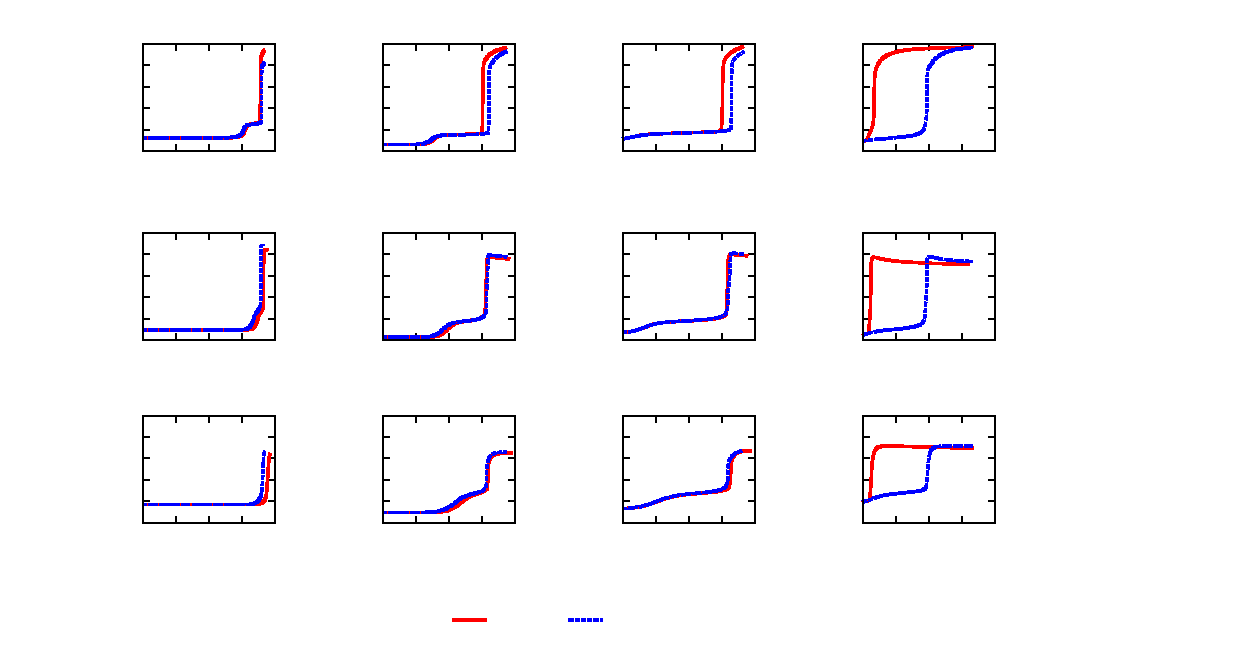
\includegraphics{LFA}}%
    \gplfronttext
  \end{picture}%
\endgroup

  \normalsize
%  \vspace{0.2in}
  \caption{Comparison between NGA and LFA results.}
  \label{fig:LFA}
\end{figure}

As shown in Fig.~\ref{fig:LFA}, two ignition stages can be seen at $Z_{\rm st}$ and $Z = 0.2$ for the $700$ K case, while at $Z = 0.3$ only one ignition dominated by low temperature chemistry is observed, due to the reduced initial temperature.   For the $800$ K case, both the flamelet and two-dimensional computation experience almost identical time histories, where two-stage ignition occurs at all three mixture fractions.  As the initial temperatures further increase, corresponding to the increase in the boundary temperatures in the CFD computation, the two-stage ignition phemonenon is less pronounced.  However, the $900$ K case still shows good argeement between the flamelet profile with the time history of the two-dimensional computation, similar to the above two cases.  
  
On the contrary, for the $1100$ K case, the ignition delay time computed with the one-dimensional flamelet assumption is significantly longer than the two-dimensional counterpart, indicating that autoignition is less important to the stabilization mechanism and that transport processes along the mixture fraction iso-contours must be important.  Noting that the scalar dissipation rate other than $\chi_{\rm st}$ is modeled through Eq.~\ref{eq:Zref}, small differences between the flamelet and CFD results are expected, even for an autoignition dominated case.  However, compared with the above three cases, the significant ignition delay at $1100$ K suggests that flame propagation dominates the stabilization of the flame structure.      

\section{Stabilization Mechanism}
With the above analysis based on species profiles, Chemical Explosive Mode Analysis, and Lagrangian Flamelet Analysis, the transition of the stabilization mechanism and the coupling between autoignition chemistry and flame propagation can be clearly identified.  In the current study, two fundamental stabilization mechanisms are relevant: the \emph {kinetic} stabilization mechanism, due to the balance between the autoignition delay time and flow residence time, and the \emph {kinematic} stabilization mechanism, due to the balance between the premixed flame propagation velocity and the local flow velocity.  

In this stratified composition and temperature field, autoignition and flame propagation are coupled through thermal and radical interactions, for the accumulation of the upstream radicals and heat release from autoignition accelerate the flame propagation velocity.  The flame also transfers heat and radicals through back diffusion processes to the upstream, which could also facilitate autoignition.

For the current study, a purely \emph {kinetically} stabilized autoignition front was not observed, for the classical triple flame structures are seen at certain locations, and the flame chemistry is dominant at the flame front.  However, as demonstrated above, the \emph {kinetic} stabilization is the dominant mechanism for the $700$ to $900$ K cases, for the steady flame structure is assisted and stabilized by autoignition.  Specifically, as seen from Fig.~\ref{fig:HRR}, the nonpremixed branch of the tribrachial flame structure has quite low heat release rate for the $700$ K case, suggesting relatively weaker flame chemistry compared to autoignition.  As the boundary temperature increases to $800$ K, an autoignition front stabilizes the multibrachial structure at rich mixture fractions, due to the shorter ignition delay time resulting from the NTC chemistry, and a modified triple flame structure stabilizes slightly downstream of this front at leaner mixture fractions.  Further increasing the boundary temperature results in higher flame propagation velocity; therefore, the flame front at leaner mixture fraction depends less on the radicals accumulation ahead of the flame and propagates upstream, although the overall structure is still stabilized \emph {kinetically}.  The transition to a \emph {kinematically} stabilized flame structure is achieved for the $1100$ K case, where the flame propagation velocity balances the local incoming flow velocity; therefore, the flame structure stabilizes close to the nozzle exit and depends least on the radical accumulation from upstream.  

Based on the understanding obtained from the current study, further extension of the stabilization regime can be made, as shown in Fig.~\ref{fig:regime}.  For fixed inlet flow velocity, when the boundary temperature is sufficiently low, the mixture cannot be autoignited, and it is essentially a frozen flow.  Even when an external ignition source is applied, the flame cannot keep up with the excessive high flow velocity, such that the flame blows off.  When the boundary temperature is high enough to activate autoignition, autoignition occurs far downstream, but the flame propagation velocity still cannot keep up with the flow velocity.  As a consequence, a pure \emph {kinetically} stabilized autoignition front can be achieved.  Due to the computational cost required for such a large domain, the purely \emph {kinetically} stabilized case was not computed.  Conversely, when the boundary temperature is sufficiently high, the flame stabilizes close to the inlet, where the upstream can be treated as frozen flow, due to reduced residence time, which is similar to the $1100$ K case.  Therefore, a purely \emph {kinematically} stabilized classical triple flame structure is achieved.  Further increase in the boundary temperature results in an attached flame with the increased flame speed.  Although not included in the current paper, an attached flame was computed at $1500$ K.  In between the purely \emph {kinetically} and \emph {kinematically} stabilized regimes, there is a transitional regime governed by both mechanisms, which corresponds to the $700$ to $900$ K cases.  Due to the NTC behavior of the autoignition chemistry, the stabilization point, in terms of mixture fraction space, varies, and the complex multibrachial flame structure appears.  

\begin{figure}[t]
  \centering
  \scriptsize
%  \vspace{-0.1in}
  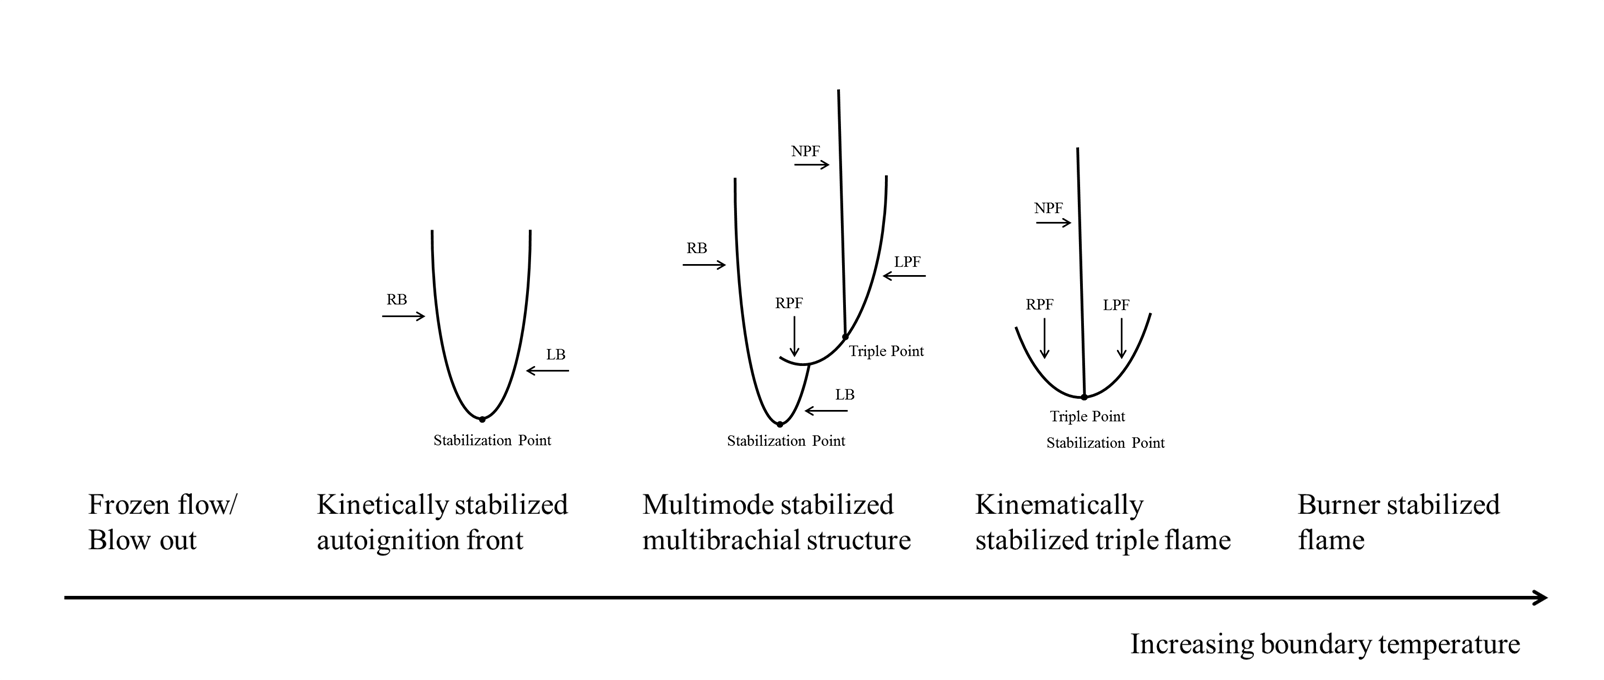
\includegraphics[width=1.0\textwidth]{regime.png}
  \normalsize
%  \vspace{-0.1in}
  \caption{Extended regimes of the stabilization mechanism as coflow boundary temperature increases.}
  \label{fig:regime}
\end{figure}


\section{Conclusions}

In the present study, two-dimensional nonpremixed DME flames in heated air coflows were computed.  The computations were conducted at $30$ atmospheres to observe the influence of NTC chemistry on the stabilization mechanism.  A uniform and fixed inlet boundary velocity was specified, and four coflow temperature ($700$, $800$, $900$, and $1100$ K) cases were studied.  The heat release rate profiles and characteristic species profiles for low and high temperature autoignition and premixed flame propagation were examined.


The heat release rate profile and characteristic species profiles for low and high temperature chemistry, autoignition, and premixed flame propagation were examined.  Further investigation based on Chemical Explosive Mode Analysis and Lagrangian Flamelet Analysis enabled the determination of the stabilization mechanism.  

The $700$ to $900$ K cases were characterized as \emph {kinetically} stabilized, due to the dominant role of autoignition chemistry.  As the boundary temperature increases, the leading point of the heat release profile shifts to richer mixture fractions and then shifts back, due to the NTC effect on the autoignition process and the coupling between autoignition and premixed flame propagation chemistry.  

The $1100$ K case was characterized as \emph {kinematically} stabilized, for it exhibits the classical triple flame structure, with stabilization achieved due to the balance between the premixed flame propagation velocity and the local incoming flow velocity.

Based on the current computational results, extended stabilization regimes were identified.  For sufficiently high inlet velocity, as the boundary temperature increases from the cold case, frozen flow is first achieved, where the mixture is nonautoignitive, and even the flame generated by an external ignition source will blow off.  When the mixture can be autoignited, the \emph {kinetically} stabilized autoignition front gradually transits to a \emph {kinematically} stabilized classical triple flame, where the premixed flame front propagation velocity balances the local incoming flow velocity.  The triple flame will eventually become attached when the boundary temperature is sufficiently high, and the flame speed is sufficiently fast.

Further study on the effects of fuel dilution and inlet velocity on the lift-off height, stabilized flame structure, and stabilization mechanism, is suggested.  For example, boundary velocity can be varied to change the flow residence time, and dilution can be added to the fuel stream to change the chemical time scale.  Moreover, if autoignition is the dominant stabilization mechanism and the scalar dissipation rate sufficiently low, the nonmonotonic lifted height variation can be observed as the boundary temperature changes, which is a plausible prediction based on the homogeneous autoignition and nonpremixed counterflow observations~\cite{deng14}.


%\section*{Acknowledgments}
%S.D., P.Z., and C.K.L. wish to acknowledge funding from the Air Force Office of Scientific Research (AFOSR), under the supervision of Dr. Mitat Birkan.


\section*{References}
\bibliographystyle{elsarticle-num-CNF}
\bibliography{DME_Jet}

\renewcommand{\thefigure}{\arabic{figure}}
\renewcommand{\thetable}{\arabic{table}}




\end{document}





  
